
\documentclass[a4paper,UKenglish,cleveref, autoref, thm-restate]{lipics-v2021}
%This is a template for producing LIPIcs articles. 
%See lipics-v2021-authors-guidelines.pdf for further information.
%for A4 paper format use option "a4paper", for US-letter use option "letterpaper"
%for british hyphenation rules use option "UKenglish", for american hyphenation rules use option "USenglish"
%for section-numbered lemmas etc., use "numberwithinsect"
%for enabling cleveref support, use "cleveref"
%for enabling autoref support, use "autoref"
%for anonymousing the authors (e.g. for double-blind review), add "anonymous"
%for enabling thm-restate support, use "thm-restate"
%for enabling a two-column layout for the author/affilation part (only applicable for > 6 authors), use "authorcolumns"
%for producing a PDF according the PDF/A standard, add "pdfa"

%\pdfoutput=1 %uncomment to ensure pdflatex processing (mandatatory e.g. to submit to arXiv)
%\hideLIPIcs  %uncomment to remove references to LIPIcs series (logo, DOI, ...), e.g. when preparing a pre-final version to be uploaded to arXiv or another public repository

%\graphicspath{{./graphics/}}%helpful if your graphic files are in another directory

\usepackage{cite}
\usepackage{amsmath,amssymb,amsfonts}
\usepackage{algorithmic}
\usepackage{graphicx}
\usepackage{bussproofs}
\EnableBpAbbreviations
\usepackage{hyperref}
\usepackage{tikz,pgfplots}
\pgfplotsset{compat=newest}
\usepackage{tikz-cd}
\usepackage{textcomp}
\usepackage{xcolor}
\usepackage{amsthm}
\usepackage{caption}
\usepackage{subcaption}
\usetikzlibrary{cd}
\usepackage{mathabx}
\usepackage{cmll}
\usepackage{stmaryrd}
\usepackage{wrapfig}
\usepackage{relsize}

\message{<Paul Taylor's Proof Trees, 2 August 1996>}
%% Build proof tree for Natural Deduction, Sequent Calculus, etc.
%% WITH SHORTENING OF PROOF RULES!
%% Paul Taylor, begun 10 Oct 1989
%% *** THIS IS ONLY A PRELIMINARY VERSION AND THINGS MAY CHANGE! ***
%%
%% 2 Aug 1996: fixed \mscount and \proofdotnumber
%%
%%      \prooftree
%%              hyp1            produces:
%%              hyp2
%%              hyp3            hyp1    hyp2    hyp3
%%      \justifies              -------------------- rulename
%%              concl                   concl
%%      \thickness=0.08em
%%      \shiftright 2em
%%      \using
%%              rulename
%%      \endprooftree
%%
%% where the hypotheses may be similar structures or just formulae.
%%
%% To get a vertical string of dots instead of the proof rule, do
%%
%%      \prooftree                      which produces:
%%              [hyp]
%%      \using                                  [hyp]
%%              name                              .
%%      \proofdotseparation=1.2ex                 .name
%%      \proofdotnumber=4                         .
%%      \leadsto                                  .
%%              concl                           concl
%%      \endprooftree
%%
%% Within a prooftree, \[ and \] may be used instead of \prooftree and
%% \endprooftree; this is not permitted at the outer level because it
%% conflicts with LaTeX. Also,
%%      \Justifies
%% produces a double line. In LaTeX you can use \begin{prooftree} and
%% \end{prootree} at the outer level (however this will not work for the inner
%% levels, but in any case why would you want to be so verbose?).
%%
%% All of of the keywords except \prooftree and \endprooftree are optional
%% and may appear in any order. They may also be combined in \newcommand's
%% eg "\def\Cut{\using\sf cut\thickness.08em\justifies}" with the abbreviation
%% "\prooftree hyp1 hyp2 \Cut \concl \endprooftree". This is recommended and
%% some standard abbreviations will be found at the end of this file.
%%
%% \thickness specifies the breadth of the rule in any units, although
%% font-relative units such as "ex" or "em" are preferable.
%% It may optionally be followed by "=".
%% \proofrulebreadth=.08em or \setlength\proofrulebreadth{.08em} may also be
%% used either in place of \thickness or globally; the default is 0.04em.
%% \proofdotseparation and \proofdotnumber control the size of the
%% string of dots
%%
%% If proof trees and formulae are mixed, some explicit spacing is needed,
%% but don't put anything to the left of the left-most (or the right of
%% the right-most) hypothesis, or put it in braces, because this will cause
%% the indentation to be lost.
%%
%% By default the conclusion is centered wrt the left-most and right-most
%% immediate hypotheses (not their proofs); \shiftright or \shiftleft moves
%% it relative to this position. (Not sure about this specification or how
%% it should affect spreading of proof tree.)
%
% global assignments to dimensions seem to have the effect of stretching
% diagrams horizontally.
%
%%==========================================================================

\def\introrule{{\cal I}}\def\elimrule{{\cal E}}%%
\def\andintro{\using{\land}\introrule\justifies}%%
\def\impelim{\using{\Rightarrow}\elimrule\justifies}%%
\def\allintro{\using{\forall}\introrule\justifies}%%
\def\allelim{\using{\forall}\elimrule\justifies}%%
\def\falseelim{\using{\bot}\elimrule\justifies}%%
\def\existsintro{\using{\exists}\introrule\justifies}%%

%% #1 is meant to be 1 or 2 for the first or second formula
\def\andelim#1{\using{\land}#1\elimrule\justifies}%%
\def\orintro#1{\using{\lor}#1\introrule\justifies}%%

%% #1 is meant to be a label corresponding to the discharged hypothesis/es
\def\impintro#1{\using{\Rightarrow}\introrule_{#1}\justifies}%%
\def\orelim#1{\using{\lor}\elimrule_{#1}\justifies}%%
\def\existselim#1{\using{\exists}\elimrule_{#1}\justifies}

%%==========================================================================

\newdimen\proofrulebreadth \proofrulebreadth=.05em
\newdimen\proofdotseparation \proofdotseparation=1.25ex
\newdimen\proofrulebaseline \proofrulebaseline=2ex
\newcount\proofdotnumber \proofdotnumber=3
\let\then\relax
\def\hfi{\hskip0pt plus.0001fil}
\mathchardef\squigto="3A3B
%
% flag where we are
\newif\ifinsideprooftree\insideprooftreefalse
\newif\ifonleftofproofrule\onleftofproofrulefalse
\newif\ifproofdots\proofdotsfalse
\newif\ifdoubleproof\doubleprooffalse
\let\wereinproofbit\relax
%
% dimensions and boxes of bits
\newdimen\shortenproofleft
\newdimen\shortenproofright
\newdimen\proofbelowshift
\newbox\proofabove
\newbox\proofbelow
\newbox\proofrulename
%
% miscellaneous commands for setting values
\def\shiftproofbelow{\let\next\relax\afterassignment\setshiftproofbelow\dimen0 }
\def\shiftproofbelowneg{\def\next{\multiply\dimen0 by-1 }%
\afterassignment\setshiftproofbelow\dimen0 }
\def\setshiftproofbelow{\next\proofbelowshift=\dimen0 }
\def\setproofrulebreadth{\proofrulebreadth}

%=============================================================================
\def\prooftree{% NESTED ZERO (\ifonleftofproofrule)
%
% first find out whether we're at the left-hand end of a proof rule
\ifnum  \lastpenalty=1
\then   \unpenalty
\else   \onleftofproofrulefalse
\fi
%
% some space on left (except if we're on left, and no infinity for outermost)
\ifonleftofproofrule
\else   \ifinsideprooftree
        \then   \hskip.5em plus1fil
        \fi
\fi
%
% begin our proof tree environment
\bgroup% NESTED ONE (\proofbelow, \proofrulename, \proofabove,
%               \shortenproofleft, \shortenproofright, \proofrulebreadth)
\setbox\proofbelow=\hbox{}\setbox\proofrulename=\hbox{}%
\let\justifies\proofover\let\leadsto\proofoverdots\let\Justifies\proofoverdbl
\let\using\proofusing\let\[\prooftree
\ifinsideprooftree\let\]\endprooftree\fi
\proofdotsfalse\doubleprooffalse
\let\thickness\setproofrulebreadth
\let\shiftright\shiftproofbelow \let\shift\shiftproofbelow
\let\shiftleft\shiftproofbelowneg
\let\ifwasinsideprooftree\ifinsideprooftree
\insideprooftreetrue
%
% now begin to set the top of the rule (definitions local to it)
\setbox\proofabove=\hbox\bgroup$\displaystyle % NESTED TWO
\let\wereinproofbit\prooftree
%
% these local variables will be copied out:
\shortenproofleft=0pt \shortenproofright=0pt \proofbelowshift=0pt
%
% flags to enable inner proof tree to detect if on left:
\onleftofproofruletrue\penalty1
}

%=============================================================================
% end whatever box and copy crucial values out of it
\def\eproofbit{% NESTED TWO
%
% various hacks applicable to hypothesis list 
\ifx    \wereinproofbit\prooftree
\then   \ifcase \lastpenalty
        \then   \shortenproofright=0pt  % 0: some other object, no indentation
        \or     \unpenalty\hfil         % 1: empty hypotheses, just glue
        \or     \unpenalty\unskip       % 2: just had a tree, remove glue
        \else   \shortenproofright=0pt  % eh?
        \fi
\fi
%
% pass out crucial values from scope
\global\dimen0=\shortenproofleft
\global\dimen1=\shortenproofright
\global\dimen2=\proofrulebreadth
\global\dimen3=\proofbelowshift
\global\dimen4=\proofdotseparation
\global\count255=\proofdotnumber
%
% end the box
$\egroup  % NESTED ONE
%
% restore the values
\shortenproofleft=\dimen0
\shortenproofright=\dimen1
\proofrulebreadth=\dimen2
\proofbelowshift=\dimen3
\proofdotseparation=\dimen4
\proofdotnumber=\count255
}

%=============================================================================
\def\proofover{% NESTED TWO
\eproofbit % NESTED ONE
\setbox\proofbelow=\hbox\bgroup % NESTED TWO
\let\wereinproofbit\proofover
$\displaystyle
}%
%
%=============================================================================
\def\proofoverdbl{% NESTED TWO
\eproofbit % NESTED ONE
\doubleprooftrue
\setbox\proofbelow=\hbox\bgroup % NESTED TWO
\let\wereinproofbit\proofoverdbl
$\displaystyle
}%
%
%=============================================================================
\def\proofoverdots{% NESTED TWO
\eproofbit % NESTED ONE
\proofdotstrue
\setbox\proofbelow=\hbox\bgroup % NESTED TWO
\let\wereinproofbit\proofoverdots
$\displaystyle
}%
%
%=============================================================================
\def\proofusing{% NESTED TWO
\eproofbit % NESTED ONE
\setbox\proofrulename=\hbox\bgroup % NESTED TWO
\let\wereinproofbit\proofusing
\kern0.3em$
}

%=============================================================================
\def\endprooftree{% NESTED TWO
\eproofbit % NESTED ONE
% \dimen0 =     length of proof rule
% \dimen1 =     indentation of conclusion wrt rule
% \dimen2 =     new \shortenproofleft, ie indentation of conclusion
% \dimen3 =     new \shortenproofright, ie
%                space on right of conclusion to end of tree
% \dimen4 =     space on right of conclusion below rule
  \dimen5 =0pt% spread of hypotheses
% \dimen6, \dimen7 = height & depth of rule
%
% length of rule needed by proof above
\dimen0=\wd\proofabove \advance\dimen0-\shortenproofleft
\advance\dimen0-\shortenproofright
%
% amount of spare space below
\dimen1=.5\dimen0 \advance\dimen1-.5\wd\proofbelow
\dimen4=\dimen1
\advance\dimen1\proofbelowshift \advance\dimen4-\proofbelowshift
%
% conclusion sticks out to left of immediate hypotheses
\ifdim  \dimen1<0pt
\then   \advance\shortenproofleft\dimen1
        \advance\dimen0-\dimen1
        \dimen1=0pt
%       now it sticks out to left of tree!
        \ifdim  \shortenproofleft<0pt
        \then   \setbox\proofabove=\hbox{%
                        \kern-\shortenproofleft\unhbox\proofabove}%
                \shortenproofleft=0pt
        \fi
\fi
%
% and to the right
\ifdim  \dimen4<0pt
\then   \advance\shortenproofright\dimen4
        \advance\dimen0-\dimen4
        \dimen4=0pt
\fi
%
% make sure enough space for label
\ifdim  \shortenproofright<\wd\proofrulename
\then   \shortenproofright=\wd\proofrulename
\fi
%
% calculate new indentations
\dimen2=\shortenproofleft \advance\dimen2 by\dimen1
\dimen3=\shortenproofright\advance\dimen3 by\dimen4
%
% make the rule or dots, with name attached
\ifproofdots
\then
        \dimen6=\shortenproofleft \advance\dimen6 .5\dimen0
        \setbox1=\vbox to\proofdotseparation{\vss\hbox{$\cdot$}\vss}%
        \setbox0=\hbox{%
                \advance\dimen6-.5\wd1
                \kern\dimen6
                $\vcenter to\proofdotnumber\proofdotseparation
                        {\leaders\box1\vfill}$%
                \unhbox\proofrulename}%
\else   \dimen6=\fontdimen22\the\textfont2 % height of maths axis
        \dimen7=\dimen6
        \advance\dimen6by.5\proofrulebreadth
        \advance\dimen7by-.5\proofrulebreadth
        \setbox0=\hbox{%
                \kern\shortenproofleft
                \ifdoubleproof
                \then   \hbox to\dimen0{%
                        $\mathsurround0pt\mathord=\mkern-6mu%
                        \cleaders\hbox{$\mkern-2mu=\mkern-2mu$}\hfill
                        \mkern-6mu\mathord=$}%
                \else   \vrule height\dimen6 depth-\dimen7 width\dimen0
                \fi
                \unhbox\proofrulename}%
        \ht0=\dimen6 \dp0=-\dimen7
\fi
%
% set up to centre outermost tree only
\let\doll\relax
\ifwasinsideprooftree
\then   \let\VBOX\vbox
\else   \ifmmode\else$\let\doll=$\fi
        \let\VBOX\vcenter
\fi
% this \vbox or \vcenter is the actual output:
\VBOX   {\baselineskip\proofrulebaseline \lineskip.2ex
        \expandafter\lineskiplimit\ifproofdots0ex\else-0.6ex\fi
        \hbox   spread\dimen5   {\hfi\unhbox\proofabove\hfi}%
        \hbox{\box0}%
        \hbox   {\kern\dimen2 \box\proofbelow}}\doll%
%
% pass new indentations out of scope
\global\dimen2=\dimen2
\global\dimen3=\dimen3
\egroup % NESTED ZERO
\ifonleftofproofrule
\then   \shortenproofleft=\dimen2
\fi
\shortenproofright=\dimen3
%
% some space on right and flag we've just made a tree
\onleftofproofrulefalse
\ifinsideprooftree
\then   \hskip.5em plus 1fil \penalty2
\fi
}

%==========================================================================
% IDEAS
% 1.    Specification of \shiftright and how to spread trees.
% 2.    Spacing command \m which causes 1em+1fil spacing, over-riding
%       exisiting space on sides of trees and not affecting the
%       detection of being on the left or right.
% 3.    Hack using \@currenvir to detect LaTeX environment; have to
%       use \aftergroup to pass \shortenproofleft/right out.
% 4.    (Pie in the sky) detect how much trees can be "tucked in"
% 5.    Discharged hypotheses (diagonal lines).

\usepackage{proof}

\bibliographystyle{plainurl}% the mandatory bibstyle



% MATH TEXT STYLES
\newcommand{\B}[1]{\mathbf{#1}}
\newcommand{\BB}[1]{\mathbb{#1}}
\newcommand{\C}[1]{\mathcal{#1}}
\newcommand{\F}[1]{\mathfrak{#1}}
\newcommand{\TT}[1]{\mathtt{#1}}
\newcommand{\RM}[1]{\mathrm{#1}}
\newcommand{\SF}[1]{\mathsf{#1}}



%CATEGORIES

\newcommand{\Met}{\mathsf{Met}}
\newcommand{\Mod}{\Lawv\mathsf{Mod}}
\newcommand{\GMet}{\Lawv\mathsf{CCat}}
\newcommand{\Fun}{\mathsf{Fun}}
\newcommand{\colim}{\mathrm{colim}}
\newcommand{\Yon}{\B{Y}}
\newcommand{\Hom}{\mathrm{Hom}}
\newcommand{\Sym}{\mathrm{Sym}}
\newcommand{\matr}[1]{\hat{#1}}

\newcommand\pfun{\mathrel{\ooalign{\hfil$\mapstochar\mkern5mu$\hfil\cr$\to$\cr}}}



% LAMBDA CALCULI

\newcommand{\lamcalc}{$\lambda$-calculus}
\newcommand{\lam}{\lambda}

\newcommand{\STLC}{\RM{STLC}}
\newcommand{\BSTLC}{\mathsf b\RM{STLC}}
\newcommand{\RSTLC}{\C R\RM{STLC}}
\newcommand{\STDLC}{\RM{ST}\partial\RM{LC}}
\newcommand{\Real}{\SF{Real}}

\newcommand{\Der}{\SF D}
\newcommand{\To}{\Rightarrow}
\newcommand{\Diff}[2]{\Der[#1,#2]}

\newcommand{\finMS}[1]{\C M_{\RM{fin}}(#1)}

\newcommand{\true}{\prog{True}}
\newcommand{\false}{\prog{False}}
\newcommand{\bool}{\SF{Bool}}

\newcommand{\Te}[1]{\C T(#1)}

\newcommand{\prog}[1]{\mathtt{#1}}




% METRIC STUFF
\newcommand{\Lawv}{\BB L}
\newcommand{\QualREL}[1]{#1 \SF{Rel}}
\newcommand{\QREL}{\QualREL{Q}}
\newcommand{\LREL}{\QualREL{\Lawv}}
\newcommand{\LCAT}{\Lawv\SF{CCat}}

\newcommand{\op}{\mathrm{op}} 
\newcommand{\sk}{\mathrm{sk}} 
\newcommand{\sym}{\mathrm{sym}} 
\newcommand{\menus}{\dotdiv} 

\newcommand{\norm}[1]{\lVert#1\rVert}
\newcommand{\supnorm}[1]{\lVert#1\rVert_\infty}
\newcommand{\absv}[1]{\left\lvert#1\right\rvert}

% TROPICAL STUFF

\newcommand{\trop}[1]{\SF t #1}
\newcommand{\model}[1]{\llbracket#1\rrbracket}
\newcommand{\nodel}[1]{\langle #1\rangle}
\newcommand{\sumt}[1]{{+}^{#1}}
\newcommand{\prodt}[1]{{\times}^{#1}}


% MISCELLANEOUS

\newcommand{\HOM}[3]{{#1}(#2,#3)}
\newcommand{\N}{\BB N}
\newcommand{\R}{\BB R}
\newcommand{\set}[1]{\{#1\}}
\newcommand{\multiset}{\C M_{\mathrm{fin}}}

\newcommand{\eps}{\epsilon}

\newcommand{\twoheaddownarrow}{\mathrel{\rotatebox[origin=c]{270}{$\twoheadrightarrow$}}\!}


%LIST ENVIRONMENTS


\newenvironment{varenumerate}
{
	\begin{list}{\arabic{numberone}.}
		{
			\usecounter{numberone}
			\setlength{\itemsep}{0pt}
			\setlength{\topsep}{0pt}
			\setlength{\parsep}{0pt}
			\setlength{\partopsep}{0pt}
			\setlength{\leftmargin}{15pt}
			\setlength{\rightmargin}{0pt}
			\setlength{\itemindent}{0pt}
			\setlength{\labelsep}{5pt}
			\setlength{\labelwidth}{15pt}
	}}
	{
	\end{list} 
}





%MATH EVIRONMENTS











\title{Tropical mathematics for the Lambda-calculus} %TODO Please add

%\titlerunning{Dummy short title} %TODO optional, please use if title is longer than one line

\author{Davide {Barbarossa}}{Dipartimento di Informatica, Universit\`a di Bologna, %[optional: Address], 
Italy% \and My second affiliation, Country 
\and \url{https://lipn.univ-paris13.fr/\~barbarossa/index.html} }{davide.barbarossa@unibo.it}{https://orcid.org/0000-0003-4608-8282}{%(Optional)Funding each author
}%TODO mandatory, please use full name; only 1 author per \author macro; first two parameters are mandatory, other parameters can be empty. Please provide at least the name of the affiliation and the country. The full address is optional. Use additional curly braces to indicate the correct name splitting when the last name consists of multiple name parts.

\author{Paolo {Pistone}}{Dipartimento di Informatica, Universit\`a di Bologna, %[optional: Address], 
Italy% \and LIP, Universit\'e de Lyon, France 
\and \url{%WebPage
} }{paolo.pistone2@unibo.it}{%Orchid
}{%(Optional)Funding each author
}


\authorrunning{D.\,Barbarossa and P.\,Pistone} %TODO mandatory. First: Use abbreviated first/middle names. Second (only in severe cases): Use first author plus 'et al.'

\Copyright{Davide Barbarossa and Paolo Pistone} %TODO mandatory, please use full first names. LIPIcs license is "CC-BY";  http://creativecommons.org/licenses/by/3.0/

\ccsdesc[500]{Theory of computation~Lambda calculus}
\ccsdesc[300]{Theory of computation~Categorical semantics}
\ccsdesc[100]{Theory of computation~Linear logic}%TODO mandatory: Please choose ACM 2012 classifications from https://dl.acm.org/ccs/ccs_flat.cfm 

\keywords{Differential lambda-calculus, Tropical semiring, Relational semantics, Lawvere quantale, Program metrics} %TODO mandatory; please add comma-separated list of keywords

\category{} %optional, e.g. invited paper

\relatedversion{} %optional, e.g. full version hosted on arXiv, HAL, or other respository/website
%\relatedversiondetails[linktext={opt. text shown instead of the URL}, cite=DBLP:books/mk/GrayR93]{Classification (e.g. Full Version, Extended Version, Previous Version}{URL to related version} %linktext and cite are optional

%\supplement{}%optional, e.g. related research data, source code, ... hosted on a repository like zenodo, figshare, GitHub, ...
%\supplementdetails[linktext={opt. text shown instead of the URL}, cite=DBLP:books/mk/GrayR93, subcategory={Description, Subcategory}, swhid={Software Heritage Identifier}]{General Classification (e.g. Software, Dataset, Model, ...)}{URL to related version} %linktext, cite, and subcategory are optional

\funding{This work has been supported by the DIAPASoN project}%optional, to capture a funding statement, which applies to all authors. Please enter author specific funding statements as fifth argument of the \author macro.

\acknowledgements{%I want to thank \dots
}%optional

%\nolinenumbers %uncomment to disable line numbering



%Editor-only macros:: begin (do not touch as author)%%%%%%%%%%%%%%%%%%%%%%%%%%%%%%%%%%
\EventEditors{John Q. Open and Joan R. Access}
\EventNoEds{2}
\EventLongTitle{42nd Conference on Very Important Topics (CVIT 2016)}
\EventShortTitle{CVIT 2016}
\EventAcronym{CVIT}
\EventYear{2016}
\EventDate{December 24--27, 2016}
\EventLocation{Little Whinging, United Kingdom}
\EventLogo{}
\SeriesVolume{42}
\ArticleNo{23}
%%%%%%%%%%%%%%%%%%%%%%%%%%%%%%%%%%%%%%%%%%%%%%%%%%%%%%

\begin{document}

\maketitle

%TODO mandatory: add short abstract of the document
\begin{abstract}
We study the interpretation of the lambda-calculus in a framework based on tropical mathematics, by considering the relational semantics weighted on the tropical semiring. The aim is to provide a framework where both program metrics, based on the analysis of program sensitivity via Lipschitz conditions, and resource analysis, based on higher-order program differentiation, coexist. In order to do that, we consider a graded-types lambda-calculus and the differential lambda-calculus, both languages ensuring bounded duplications.
A typical result of such line of research is that, thanks to the tropical operations, a simply typed term is interpreted as a locally Lipschitz map, which is in turn decomposed as an inf of more and more sensitive Lipschitz ones, corresponding to the interpretations of the approximants given by the lambda-calculus Taylor expansion.
We finally describe some promising lines of research, showing in particular how such tropical model expresses natural optimisation problems of probabilistic calculi.
\end{abstract}

\section{Two kinds of quantitative approaches}

In recent years, more and more interest in the programming language community has been directed towards the study of \emph{quantitative} properties of programs like computing the number of computation steps or convergence probabilities, 
as opposed to purely \emph{qualitative} properties like termination or program equivalence. 
Notably, a significant effort has been made to extend, or adapt, well-established qualitative methods, like type systems, relational logics or denotational semantics, to account for quantitative properties. We can mention, for example, 
intersection type systems aimed at capturing time or space resources \cite{decarvalho2018, Accattoli2022} or convergence probabilities \cite{Breuvart2018, PistoneLICS2022},  relational logics to account for probabilistic properties like e.g.~differential privacy \cite{Barthe_2012} or metric preservation \cite{Reed2010, dallago}, as well as the study of denotational models for 
probabilistic \cite{Ehrhard2011, Staton2017} or differential \cite{difflambda} extensions of the $\lambda$-calculus. 
The main reason to look for methods relying on (quantitative extensions of) type-theory or denotational semantics is that these approaches yield \emph{modular} and \emph{compositional} techniques, that is, allow one to deduce properties of complex programs from the properties of their constituent parts.   

\subsection{Two kinds of quantitative approaches}

Among such quantitative approaches, two different directions have received considerable attention. 

On the one hand one there is the approach of \emph{program metrics} \cite{Reed2010, Gaboardi2017, Gabo2019} and \emph{quantitative equational theories} \cite{Plotk}: when considering probabilistic or approximate computation, rather than asking whether two programs compute \emph{the same} function, it makes more sense to ask   whether they compute functions which do not differ \emph{too much}. This has motivated the study of denotational frameworks in which types are endowed with a metric, measuring similarity of behavior; this approach has found  applications in e.g.~differential privacy \cite{Reed2010} and coinductive methods \cite{Bonchi2018}, and was recently extended to account for the full $\lambda$-calculus \cite{Geoffroy2020, PistoneLICS, PistoneFSCD2022}.

On the other hand, there is the approach based on \emph{differential} \cite{difflambda} or \emph{resource-aware} \cite{Boudol1993} extensions of the $\lambda$-calculus, which is well-connected to the so-called \emph{relational semantics} \cite{Manzo2012, Manzo2013, dill} and has a syntactic counterpart in the study of \emph{non-idempotent} intersection types \cite{decarvalho2018, Mazza2016}. This family of approaches have been exploited to account for higher-order program differentiation \cite{difflambda}, to establish reasonable \emph{cost-models} for the $\lambda$-calculus \cite{Accattoli2021}, and have also been shown suitable for the probabilistic setting \cite{Manzo2013, Breuvart2018, PistoneLICS2022}. 


In both approaches the notion of \emph{linearity}, in the sense of linear logic \cite{girardLl} (i.e.~of using inputs exactly once), plays a crucial role.
In metric semantics, linear programs correspond to \emph{non-expansive} maps, that is, to functions that do not increase distances; moreover, the possibility of duplicating inputs leads to interpret \emph{bounded} programs (i.e.~programs with a fixed duplication bound) as \emph{Lipschitz-continuous} maps \cite{Gaboardi2017}.
By contrast, in the standard semantics of the differential $\lambda$-calculus, linear programs correspond to linear maps, in the usual algebraic sense, while the possibility of duplicating inputs leads to consider functions defined as \emph{power series}.


A natural question is thus whether these two apparently unrelated ways of interpreting linearity and duplication can be somehow reconciled. At a first glance, there seems to be a  ``logarithmic'' gap between the two approaches:
in metric models $n$ times duplication results in a \emph{linear} (hence Lipschitz) function $n\cdot x$, while in differential models this results in a \emph{polynomial} function $x^{n}$, hence not Lipschitz. The fundamental motivation of this work is then the observation that 
this gap is naturally overcome once we interpret these functions in the framework of tropical mathematics, where, as we'll see, the monomial $x^{n}$ precisely reads as the linear function $n\cdot x$.

% from higher-order programs is based on  soon as one develops  differential semantics in the framework of 
%tropical mathematics.
%
%''
%
%s
%emantics a typical ``duplicating'' map is obtained by composing the diagonal with multiplication:
%$$
%\begin{tikzcd}
%\mathbb R \ar{rrr}{x\mapsto \langle x, x\rangle}
% & &  &
% \mathbb R\times \mathbb R 
% \ar{rrr}{\langle x,y\rangle \mapsto x\cdot y}
% & & & \mathbb R
%\end{tikzcd}
%$$
%yielding the square product function $\lambda x.x^{2}$.
%However, in metric semantics this function needs not even exist (as these models are often restricted to Lipschitz-continuous maps \cite{Gabo2017})! Instead, a typical ``duplicating'' map can be obtained by composing the diagonal with the sum 
%$$
%\begin{tikzcd}
%\mathbb R \ar{rrr}{x\mapsto \langle x, x\rangle}
% & &  &
% \mathbb R\times \mathbb R 
% \ar{rrr}{\langle x,y\rangle \mapsto x+y}
% & & & \mathbb R
%\end{tikzcd}
%$$
%yielding the linear (and Lipschitz) function $\lambda x.2x$.
%
%As this example seems to suggest, there seems to be a sort of ``logarithmic'' gap between the two approaches. Can this be made explicit?



\subsection{Tropical mathematics and program semantics } 


Tropical mathematics was introduced in the seventies by the Brazilian mathematician Imre Simon \cite{Simon} as an alternative approach to algebra and geometry where the usual ring structure of numbers based on addition and multiplication is replaced by the semiring structure given, respectively, by ``$\min$'' and ``$+$''.
%
%
% interpreting the usual ``$\times$'' and  ``$+$'' operations by  ``$+$'' by ``$\min$''. It can thus be seen as a sort of ``logarithmic'' version of usual geometry (this idea can be made precise via the so-called \emph{Maslov deformation} \cite{}).
%Tropical mathematics is a form of \emph{idempotent} mathematics, since the role of addition is 
%played by the idempotent operation $\min$.
For instance, the polynomial $p(x,y)=x^{2}+xy^{2}+y^{3}$, when interpreted over the tropical semiring, translates as the piecewise linear function
$
\varphi(x,y)=\min\{2x, x+2y, 3y\}
$.

%This is not a \emph{ad-hoc} setting: 
In the last decades, tropical geometry evolved into a vast and rich research domain, providing a combinatorial counterpart of usual algebraic geometry, with important connections with optimisation theory \cite{Sturmfelds}.
Computationally speaking, working with $\min$ and $+$ is generally easier than working with standard addition and multiplication; for instance, the fundamental (and generally intractable) problem of finding the roots of a polynomial admits a \emph{linear time} algorithm in the tropical case (and, moreover,  the tropical roots can be used to approximate the actual roots \cite{Noferini2015}).
The computational nature of tropical notions explains why these are so widely applied in computer science, notably for convex analysis and machine learning (see \cite{Maragos2021} for a recent survey).

Coming back to our discussion on program semantics, tropical geometry might seem to provide precisely what look for, as it turns the monomials $x^{n}$ into the Lipschitz map  $n\cdot x$.
At this point, it is worth mentioning that a tropical variant of relational semantics has already been considered \cite{Manzo2013}, and shown capable of capturing \emph{best-case} quantitative properties, but has not yet been studied in detail. Furthermore, connections between tropical linear algebra and metric spaces have also been observed \cite{Fuji} within the abstract setting of \emph{quantale-enriched} categories \cite{Hofmann2014, Stubbe2014}.
However, a thorough investigation of the interpretation of the $\lambda$-calculus within tropical mathematics has not yet been undertaken. 

In this paper we demonstrate that the relational interpretation of the $\lambda$-calculus based on tropical mathematics does indeed provides the desired bridge between differential and metric semantics. Moreover, we show that the conceptual unification of these two approaches suggests ways in which techniques from resource-analysis could be used in sensitivity analysis and \emph{vice-versa}, paving the way for new  applications of tropical geometry to the  study of higher-order programs.


\subsection{Contributions}

Our contributions in this paper are threefold:
\begin{itemize}

\item we study the relational model over the tropical semiring  and we show that the functions interpreting simply-typed lambda terms, which correspond to a generalization of \emph{tropical Laurent series} \cite{Porzio2021}, are locally Lipschitz-continuous, thus yielding a full-scale metric semantics for the $\lambda$-calculus and its bounded fragments. This is in Sections \ref{section3} and \ref{section4}.
%Moreover, we exploit the differential structure of the relational model to study the \emph{tropical Taylor expansion} of a $\lambda$-term, which can be seen as an approximation of the term by way of Lipschitz-continuous maps.


\item Using the relational model as our main source of inspiration,  we suggest a few potential applications of tropical methods to the study of quantitative properties of non-deterministic and probabilistic functional programs, like counting best-case computation steps, 
measuring convergence log-probabilities, and 
differential privacy. This is in Section~\ref{section5}

\item We conclude 
by putting the connection between the 
tropical, differential and metric viewpoints at the right level of generality.
By recalling and suitably extending a well-known correspondence between Lawvere's \emph{generalized metric spaces} \cite{Lawvere1973, Stubbe2014} and modules over the tropical semi-ring \cite{Russo2007}, we show that the category of \emph{complete} generalized metric spaces provides a model of the differential $\lambda$-calculus which extends the tropical relational model. This is in Section~\ref{section6}.
\end{itemize}
%
%\section{Bounded and Differential $\lambda$-Calculi}
%
%
%Bounded Simply Typed $\lambda$-calculus $\BSTLC$:
%$$
%A::= o \mid !_{n}A \multimap A
%$$
%
%
%Resource Simply Typed $\lambda$-calculus $\RSTLC$:
%$$
%A::= o \mid [A, \dots , A] \multimap A
%$$
%
%
%Define a translation of types $(-)^{\C R}$ from $\BSTLC$ to $\RSTLC$ by $o^{\C R}=o$ and $(!_{n}A\multimap B)^{\C R}=
%[\underbrace{A^{\C R},\dots, A^{\C R}}_{n\text{ times}}]\multimap B^{\C R}$.
%
%\begin{proposition}
%$\Gamma \vdash_{\BSTLC} M:A$ implies 
%$\Gamma^{\C R}\vdash_{\RSTLC}M:A^{\C R}$.
%\end{proposition}
%





\section{The category $\LREL$}\label{section3}


%
%Fino a qui niente a capo
%
%Fino a qui niente a capo
%
%Fino a qui niente a capo
%
%Fino a qui niente a capo
%
%Fino a qui niente a capo
%
%Limite! Alla prossima riga sforo oltre 12 pag.
%

%In the next section we recall some basic ideas from tropical mathematics, and its connection with the study of the Lawvere quantale.
%Since polynomials correspond to piecewise linear (hence Lipschitz) functions in tropical mathematics,
%The reconstruction of the relational semantics over the tropical semi-ring, presented in Section \ref{section3} and Section \ref{section4}, will provide a metric semantics of the differential $\lambda$-calculus, bridging sensitivity and resource analysis. 
%In Section \ref{section5} we suggest potential applications of this approach, relating well-studied applications of program metrics, resource analysis with current uses of tropical mathematics in computer science.  
%Finally, in Section \ref{section6} we show that the connection between the metric and differential analysis of higher-order programs extends well beyond the relational semantics, through a more abstract correspondence between {generalized metric spaces} and modules over the tropical semiring.


%At the basis of our approach is the observation that the \emph{tropical semiring} $([0,\infty], \min, +)$, which is at the heart of tropical mathematics, coincides with the \emph{Lawvere quantale} $\Lawv=([0,\infty], \geq, +)$ \cite{Hofmann2014, Stubbe2014}, the structure at the heart of the categorical study of metric spaces initiated by Lawvere himself \cite{Lawvere1973}.
%Let us recall that a quantale is a complete lattice endowed with a continuous monoid action. In the case of $\Lawv$ the lattice is defined by the reverse order $\geq$ on $\BB R$, and the monoid action is provided by addition. Notice that the lattice join operation of $\Lawv$ coincides with the idempotent semiring operation $\min$. 
%A consequence of these observations is that, as we discussed below, the tropical approach to linear algebra coincides with the study of ``$\Lawv$-valued matrices'', i.e.~of maps of the form $s: X\times Y\to \Lawv$ .
%In particular, a (possibly $\infty$) metric on a set $X$ is nothing but a ``$\Lawv$-valued square matrix'' $d:X\times X\to \Lawv$ satisfying axioms like e.g.~the triangular law (indeed, such distance matrices correspond to $\Lawv$-\emph{enriched categories}, a viewpoint we explicitly take in Section \ref{section6}). 

%The study of matrices with values over the tropical semiring can be seen as a special case of the \emph{quantitative relational semantics} \cite{Manzo2013}, a well-studied semantics of the $\lambda$-calculus. 

A \emph{continuous} semiring \cite[Def. II.5]{Manzo2013} is a cpo equipped with an order-compatible semiring structure.
In a continuous semiring, all series always converge as $\sup$ of its partial sums.
%This is crucial for the definition of the weighted relational models for the $\lambda$-calculus.

\begin{example}
$[0,\infty]$ is a continuous semiring, which we denote $\overline{R_{\geq 0}}$, with usual order and semiring structure.
Notice that $\infty$ is added to ``artificially'' force any infinite series to converge.
The continuous semiring that we will use throughout all this paper is (one of) the so-called \emph{tropical semiring} $\Lawv:=[0,\infty]$ with $\min$ as sum (notice that it is idempotent) and $+$ as product.
Not only $\Lawv$ is at the heart of tropical mathematics, but it also coincides with the \emph{Lawvere quantale} \cite{Hofmann2014, Stubbe2014}
%(remember that a quantale is a complete lattice, for $\Lawv$ the order is $\geq$, endowed with a continuous monoidal action, for $\Lawv$ it is $+$)
, the structure at the heart of the categorical study of metric spaces initiated by Lawvere himself \cite{Lawvere1973}. 
%Notice that the lattice join operation of $\Lawv$ coincides with the idempotent semiring operation $\min$. 
\end{example}

For $Q$ a continuous semiring, one lets the category $\QREL$ (\cite{Manzo2013} calls it $Q^\Pi$) have sets as objects and set-indexed matrices with coefficients in $Q$ as morphisms, i.e.~$\QREL(X,Y):=Q^{X\times Y}$.
%The identity morphism of $\QREL$ is the identity matrix $I\in Q^{X\times X}$,
% given by $i_{a,a}=1$ and $i_{a,b\neq a}=0$, and
The composition $st\in Q^{X\times Z}$ of $t\in Q^{X\times Y}$ and $s\in Q^{Y\times Z}$ is given by $(st)_{a,c}:=\sum_{b\in Y} s_{b,c}t_{a,b}$ (such series converges because $Q$ is continuous).
As expected, $Q^X$ is a $Q$-semimodule and we identify $\HOM{\QREL}{X}{Y}$ with the set of linear maps from $Q^X$ to $Q^Y$, which have shape $f(x)_b=:\sum_{a\in X} \matr f_{a,b}x_a$, for some matrix $\matr f\in Q^{X\times Y}$.
% \begin{remark}
 %Following \cite{Manzo2013, Hofmann2014, Ehrhard2005}, we chose to see a matrix $t$ from $X$ to $Y$ as a map $t:X\times Y\to Q$.
% 
% fix $\HOM{\QREL}{X}{Y}:=Q^{X\times Y}$ with composition $st:X\times Z\to Q$ of $s:Y\times Z\to Q$ and $t:X\times Y\to Q$ defined by $(st)_{a,c}:=\sum_{b\in Y} s_{b,c}t_{a,b}$.
Notice that usual linear algebra conventions correspond to work in $\QREL^{\op}$, %a matrix $X\times Y\to Q$ is usually called a ``$Y\times X$-matrix'', meaning $Y$ rows and $X$ columns
e.g.\ the usual matrix-vector product defines a map $Q^Y\to Q^X$.
Following \cite{Manzo2013, Hofmann2014, Ehrhard2005}, we are instead working with transpose matrices.
%\end{remark}
%
%In $\QREL^{op}$ (which corresponds to systematically taking transpose matrices), composition coincides with the product matrix/matrix and $\hat{(\cdot)}$ with the product matrix/vector.
%In order to avoid confusion, we will refer to a $t\in Q^{X\times Y}$ just as a \emph{matrix from $X$ to $Y$}.
%
%
%
%We must fix a convention for matrices: following \cite{Manzo2013, Hofmann2014, Ehrhard2005}, we fix $\HOM{\QREL}{X}{Y}:=Q^{X\times Y}$ with composition $st:X\times Z\to Q$ of $s:Y\times Z\to Q$ and $t:X\times Y\to Q$ defined by $(st)_{a,c}:=\sum_{b\in Y} s_{b,c}t_{a,b}$.
%In linear algebra, a map $X\times Y\to Q$ is usually called a ``$Y\times X$-matrix'', meaning $Y$ rows and $X$ columns.
%In particular, the product of such a matrix for a vector defines a map $Q^Y\to Q^X$.
%Instead, we prefer to see a $t\in\HOM{\QREL}{X}{Y}$ as giving rise to a map $\hat t:Q^X\to Q^Y$ defined by $\hat t(x)_a:=\sum_{b\in Y} t_{a,b}x_a$.
%In $\QREL^{op}$ (which corresponds to systematically taking transpose matrices), composition coincides with the product matrix/matrix and $\hat{(\cdot)}$ with the product matrix/vector.
%In order to avoid confusion, we will refer to a $t\in Q^{X\times Y}$ just as a \emph{matrix from $X$ to $Y$}.
%As it is expected, $Q^X$ is a $Q$-semimodule and the bijection $\hat{(\cdot)}$ identifies $\HOM{\QREL}{X}{Y}$ with the set of linear maps from $Q^X$ to $Q^Y$.

The main actor of this paper is the category $\LREL$. % of sets and matrices with values over $\Lawv$ (which is a continuous semi-ring).
%, where $\Lawv$ is the already introduced Lawvere quantale, seen as the idempotent complete semiring $(\BB R_{\geq0}\cup\set{\infty},\inf,\infty,+,0)$.
%The category $\LREL$ is well-defined because $\Lawv$ is a continuous semiring (w.r.t.\ its quantale order $\preceq$.
%This amounts to check that $\min$ and $+$ commute with the $\inf$ (as operations on $\BB R_{\geq0}\cup\set{\infty}$, which is immediate), and that $(\Lawv,\preceq)$ is a cpo with $\infty$ as bottom element (which is immediate since in $\Lawv$ we have $\vee = \inf$) .
It is worth observing that the composition in $\LREL$ %is the tropicalisation of the one defining it in $\QREL$, i.e.
reads as \ $(st)_{a,c}:=\inf_{b\in Y}\set{s_{b,c}+t_{a,b}}$;
similarly, the linear functions $f:\Lawv^X\to \Lawv^Y$, %induced by matrices
which we call \emph{tropical linear}, are exactly those of shape $f(x)_b=\inf_{a\in X} \set{\matr f_{a,b}+x_a}$, for some $\matr f\in\Lawv^{X\times Y}$.
%\end{remark}

%Since $\Lawv$ is a continuous commutative semiring, [Proposition III.3, \cite{Manzo2013}] immediately applies and gives:

%\begin{proposition}
% $\LREL$ is a linear $\Lawv$-category.
%\end{proposition}

%Unwrapping [Definition II.9, \cite{Manzo2013}], this means that:
%$\HOM{\LREL}{X}{Y}$ is a continuous $\Lawv$-semimodule, with semimodule operations defined pointwise;
%$\LREL$ is a continuous $\Lawv$-category, i.e.\ composition of morphisms commutes with $\inf$'s;
%$\LREL$ is linear, i.e.\ pre- and post-composition with any morphism in any $\HOM{\LREL}{X}{Y}$ are automorphisms on it.

%In the next sections we will see how $\LREL$ gives rise to denotational models of several variants of the $\lam$-calculus.



%
%
%
% 

%
%
%or more generally as a power series $f(x)=\sum_{n}\widehat f_{n}x^{n}$ with coefficient $\widehat f_{n}\in [0,1]$, we can define its \emph{tropicalization} $\trop f: \Lawv \to \Lawv$ as the function 
%\begin{align}
%\trop f(\alpha)= \inf_{n}\left\{ 
%\end{align}
%
%This correspondence can be made precise through the the so-called
% \emph{de Maslov dequantization} \cite{}.
% For each positive real $t$, any polynomial in $\BB R[x]$ can be written under the \emph{$t$-parameterized} form:
% \begin{align}
% p_{t}(x)= \sum_{i=1}^{k}t^{c_{i}}x^{i}
% \end{align}
% with the coefficients $c_{i}$ taken from $\Lawv$. 
% It is clear then that tropical polynomials and $t$-parameterized polynomials admit a one to one correspondence between their presentations.
% 
% Actually, the $\varphi$s and the $p_{t}$s can be related by passing through some intermediate functions $\varphi_{t}$ introduced by Maslov.
%For any $t>1$, the functions $\phi_{t}(x)=-\log_{t}x$ and $\psi_{t}(\alpha)=t^{-\alpha}$ are inverse of each other and define thus continuous (w.r.t.\ the usual topologies) bijections between the space of probabilities $[0,1]$ and $\BB R_{\geq 0}\cup\set{\infty}$ (we write $\log$ for the natural logarithm).
%Moreover, if we set $\alpha \widetilde+ \beta:= \frac{\alpha+\beta}{2}$, $\alpha\sumt{t}\beta=\phi_{t}(\psi_{t}(\alpha)\widetilde{+}\psi_{t}(\beta))=-\log (e^{-\alpha/t}+e^{-\beta/t})-\phi_{t}(2)$ and $\alpha\prodt{t} \beta:=\phi_{t}(\psi_{t}(\alpha)\psi_{t}(\beta))=\alpha+\beta$, it is known that: $\lim_{t\to 0}\alpha\sumt{t} \beta= \min\{\alpha,\beta\}$.
%In this sense, setting $\Lawv_t:=([0,\infty],\sumt{t},\prodt{t})$, one says that $\Lawv_t\to_{t\to 0^+}\Lawv$.
%Moreover, setting $\widetilde\Lawv:=([0,\infty],\widetilde+,\cdot)$, it can be shown that $\Lawv_t\simeq\widetilde\Lawv$ for all $t>0$, so the $\Lawv_t$ are all isomorphic, whereas at the limit we have a discontinuity: it can be shown that $\Lawv_t\not\simeq\Lawv$.
% 

%
%{\color{red}Lista delle cose da dire:}
%
%1) Def di quantale, come lattice e come complete idempotent semiring.
%Among the the so-called \emph{tropical semirings}, we consider the \emph{Lawvere quantale/semiring}.
%
%2) Def di $\Lawv$, the \emph{Lawvere quantale}: seen as the idempotent complete semiring, it is $(\BB R_{\geq0}\cup\set{\infty},\inf,\infty,\cdot,0)$.
%Seen as lattice it is defined by the order $\preceq$, which is the reversed order $\geq$ of the usual order $\leq$ on $\BB R_{\geq0}\cup\set{\infty}$.
%
%3) Maslov dequantisation:
%
%First, let us recall that for any non-negative real $t$, the functions $\phi_{t}(x)=-t\log x$ and $\psi_{t}(\alpha)=e^{-\alpha/t}$ are inverse of each other and define thus continuous (w.r.t.\ the usual topologies) bijections between the space of probabilities $[0,1]$ and $\BB R_{\geq 0}\cup\set{\infty}$ (we write $\log$ for the natural logarithm).
%Moreover, if we set $\alpha \widetilde+ \beta:= \frac{\alpha+\beta}{2}$, $\alpha\sumt{t}\beta=\phi_{t}(\psi_{t}(\alpha)\widetilde{+}\psi_{t}(\beta))=-\log (e^{-\alpha/t}+e^{-\beta/t})-\phi_{t}(2)$ and $\alpha\prodt{t} \beta:=\phi_{t}(\psi_{t}(\alpha)\psi_{t}(\beta))=\alpha+\beta$, it is known that: $\lim_{t\to 0}\alpha\sumt{t} \beta= \min\{\alpha,\beta\}$.
%In this sense, setting $\Lawv_t:=([0,\infty],\sumt{t},\prodt{t})$, one says that $\Lawv_t\to_{t\to 0^+}\Lawv$.
%Moreover, setting $\widetilde\Lawv:=([0,\infty],\widetilde+,\cdot)$, it can be shown that $\Lawv_t\simeq\widetilde\Lawv$ for all $t>0$, so the $\Lawv_t$ are all isomorphic, whereas at the limit we have a discontinuity: it can be shown that $\Lawv_t\not\simeq\Lawv$.
%
%4) Def di $\trop$ di un polinomio/serie, (\`e la stessa formula, dipende solo se gli indici sono finiti/infiniti).
%Come sta scritto sotto, giusto un po' pi\`u formale (per esempio, scriverlo come Definizione).
%
%The fundamental observation that led to the study of mathematics over the \emph{tropical semi-ring} $\Lawv=([0,\infty],\min,+)$ was that, by replacing everywhere the ``$+$'' by the ``$\min$'' and the ``$\times$'' by the ``$+$'', many algebraic and geometric objects becomes combinatorial and their computation simpler. 
%
%For instance, the tropicalization of a cubic polynomial $p(x)=ax^{3}+bx^{2}+cx+d$ yields a piecewise-linear function 
%\begin{align}
%\trop p(\alpha)= \min\{ 3\alpha+a, 2\alpha+b, \alpha+c,d\}
%\end{align}
%Notably, the \emph{tropical roots} (whose definition is recalled in Section \ref{section3}) of $\trop p(\alpha)$ can be found through a rather simple (indeed polytime \cite{}) algorithm, and can be used to \emph{approximate} the actual roots of $p(x)$ \cite{}. 
%More generally, the tropicalization of a power series $f(x)=\sum_{n}\widehat f_{n}x^{n}$ yields a \emph{tropical Laurent series} \cite{} 
%\begin{align}
%\trop f(\alpha)= \inf_{n}\left\{n\alpha+ \widehat f_{n}\right\}
%\end{align}
%a class of functions that we will study in detail in Section \ref{section4}.
%
%%- generalities about tropical maths (tropicalisation $\trop P$  of polynomials and of Laurent series, and their roots -- all that without $\LREL$)
%


\subsection{... As (weighted relational) model of several $\lambda$-calculi}
The category $\LREL$ satisfies many nice properties which make it able to model all the variants of the $\lambda$-calculi to which we are interested in here. Although the majority of such properties are shared with the general class of models of $\lambda$-calculi called \emph{weighted relational models}, thoroughly studied in \cite{Manzo2013}, we mention them for our particular case in order to highlight how these look like in the tropical setting, but also to make the non-expert in such topics reader able to follow.
The real interest in our particular model will come in the next \autoref{sec:tls}.

\paragraph{Prohibited duplication/erasure: the \emph{linear} $\STLC$}\label{sec:3A}[Section III.A, Weighted], immediately gives:

\begin{fact}\label{fact:LREL_SMCC}
 $\LREL$ is a Symmetric Monoidal Closed Category.
\end{fact}

Its monoidal structures is given by a tensor product $\otimes$ acting on the objects as the Cartesian product of sets, and as the Kronecker product of matrices on morphisms.
Its closed structures is given by $X\multimap Y:=X\times Y$ with the usual evaluation and curry morphisms yielding a symmetric monoidal adjunction: $\LREL(Z\otimes X, Y) \simeq \LREL (Z, X\multimap Y)$.

Fact~\ref{fact:LREL_SMCC} means that $\LREL$ is a model of Intuitionistic Multiplicative Linear Logic (IMLL), and thus we can interpret \emph{linear} $\lam$-terms in it.

 {\color{red}spiegare linear lambda e tra parentesi IMLL}


\paragraph{Allowed duplication/erasure: the $\STLC$}\label{sec:3B}%\subsubsection{Unbounded duplications}

If in the previous subsection we considered \emph{bounded} multisets via the graded comonad $(!_n)_{n\in\N}$, it is immediate to see that \emph{unbounded} multisets yield a comonad able to interpret the $\STLC$:
following [Corollary III.6, Weighted] we have:

\begin{fact}
 $\LREL$ is Lafont.
\end{fact}

Therefore, it is well known that the map $X\mapsto \finMS{X}$ lifts to a functor $!:\LREL\to\LREL$ which %satisfies the adjunction $\LREL(!(Z\& X),Y) \simeq \LREL(!Z, !X\multimap Y)$, at 
is a Lafont-exponential.
In particular, [Theorem III.7, Weighted] says that:
\begin{fact}
 The coKleisli $\LREL_!$ is CCC, i.e.\ a model of $\STLC$.
\end{fact}

It is instructive at this point to see what its CCC-structure looks like in our tropical world.
In particular, the coKleisli composition of $s\in\Lawv^{!Y\times Z}$ and $t\in\Lawv^{!X\times Y}$ is the matrix $s\circ_! t\in\Lawv^{!X\times Z}$ where $(s\circ_! t)_{\mu,c}$ is:
\[
 \inf\limits_{n\in\N, b_1\dots,b_n\in Y, \mu = \mu_1*\cdots *\mu_n}
 \set{s_{[b_1,\dots,b_n],c} + \sum\limits_{i=1}^n t_{\mu_i,b_i}}.
\]
The exponential object $X\multimap Y$ is $!X+Y$ (where $+$ is the disjoint union).
Remember that in $\Lawv$ the neutral element for addition is $\infty$ and the neutral for multiplication is $0$, so for instance the evaluation map is the matrix $\RM{eval}^{X,Y}\in\Lawv^{!((X\multimap Y) + X)\times Y}\simeq\Lawv^{(!!X\times !Y\times !X)\times Y}$ given by $\RM{eval}^{X,Y}_{\rho_1\oplus\rho_2\oplus\mu,b}:=0$ if $\rho_1=[\mu]$ and $\rho_2=[b]$, and $\RM{eval}^{X,Y}_{\rho_1\oplus\rho_2\oplus\mu,b}:=\infty$ otherwise.

\begin{remark}[Tropical Laurent series]
 As usual, a matrix $t\in\HOM{\LREL_!}{X}{Y}$ operates as a linear map $\widehat t:\Lawv^{!X}\to\Lawv^Y$.
 But we can also ``express it in the base $X$'', i.e.\ see it as a map $t^!:\Lawv^X\to\Lawv^Y$, by setting $t^!(x):=t\circ_! x$ (we are identifying $\Lawv^X$ with the set $\HOM{\LREL_!}{\emptyset}{X}$ of the \emph{points} of $X$).
 This is the notion of \emph{non-linear} map generated by the CCC-structure of $\LREL_!$.
 Concretely, we have:
 \[t^!(x)_b=\inf\limits_{\mu\in !X} \set{\mu x+ t_{\mu,b}}\] where $\mu x:=\sum\limits_{a\in X} \mu(a)x_a$.
 Since in the general case of $\QREL$, $t^!$ is a Laurent series with operations in $Q$, let us call \emph{tropical Laurent series} the functions of shape $t^!$ for some $t\in\HOM{\LREL_!}{X}{Y}$.
\end{remark}

\begin{remark}
 Indentifying $!\set{*}\simeq \N$ and $\Lawv^{\set{*}}\simeq\Lawv$, the tropical Laurent series generated by the morphisms in $\HOM{\LREL_!}{\set{*}}{\set{*}}$ are exactly the functions $f:\Lawv\to\Lawv$ of shape $f(x)=\inf\limits_{n\in\N}\set{nx+\widehat f(n)}$, for some $\widehat f:\N\to\Lawv$.
Remark that we find usual \emph{tropical polynomials} of tropical geometry as a particular case: they corrispond to the ones for which the support $\set{n\in\N\mid\widehat f(n)\neq\infty}$ of $\widehat f$ is \emph{finite}.
\end{remark}

\begin{proposition}\label{prop:descrete}
 The interpretation $\model M$ of a $\lam$-term $M$ in $\LREL$ is a \emph{descrete} matrix, i.e.\ its coefficients are either $0$ or $\infty$.
\end{proposition}
\begin{proof}
 First easily prove that composition preserves descreteness.
 Then go by straightforward induction on $M$, using that the projections and evaluation of  $\LREL$ are descrete.
\end{proof}

The fact that ordinary $\lam$-terms become only descrete matrices may seem a restrictive property.
In Section~\ref{sec:app} we will however discuss how we can use this model in order to make it keep track of quantitative effects of programs.

\begin{example}\label{ex:famous_ex}
 The function $f:\Lawv\to\Lawv$, $f(x):=\inf\limits_{n\in\N}\set{nx+\frac{1}{2^n}}$ is a tropical Laurent series: it is of shape $f=t^!$, for $t\in\Lawv^{!\set{*}\times\set{*}}$, $t_{\mu,*}:=2^{-\# \mu}$.
By Proposition~\ref{prop:descrete}, $f$ is not the interpretation of a $\lam$-term, because its matrix is not descrete. Therefore $\LREL_!$ is not a full-complete model of $\STLC$.
\end{example}

\begin{remark}\label{rmk:ModelsOfBSTLC}
It is known {\color{red}(([reference??] e dire meglio)} that the maps $X\mapsto \C M_{\leq n}(X)$ ($n\in\BB N$) lift to functors $!_n:\LREL\to\LREL$.
The sequence $(!_n)_{n\in\N}$ can be then turned into a $\N$-graded linear exponential comonad on (the SMC) $\LREL$, satisfying the adjunction:
$\LREL(Z\otimes !_{n}X,Y) \simeq \LREL(Z, !_{n}X\multimap Y)$.
Therefore, $\LREL$, together with $(!_n)_{n\in\N}$, is a model for $\BSTLC$. 
Concretely, a type %$A::= o \mid !_{n}A \multimap A$
{\color{red}(i tipi meglio dirli in Section II)} is in interpreted as $\model o=\B 1$ and 
$\model{!_{n}A\multimap B}:= \C M_{\leq n}(\model A) \times \model B$.
\end{remark}
%Bounded types are interesting because of the following proposition:
%\begin{proposition}
%For all bounded types $A,B$, the morphisms from $\model A$ to $\model B$ (in all parametric relational models) correspond to polynomials.
%\end{proposition}
%\begin{proof}
%It suffices to check that $\model A$ is finite for all bounded types $A$. Indeed this implies that a morphism $t:\model A\to \model B$ is a finite matrix $t: \model A \times \model B \to \Lawv$.Hence, its corresponding map $\widehat t:\Lawv^{\model A} \to \Lawv^{\model B}$ is a polynomial.
%\end{proof}

%For example (here $!_{n}(\Lawv^{X}):= \Lawv^{\C M_{\leq n}(X)}$):
%\begin{itemize}
%\item a map $f\in \LREL( !_{1}\Lawv, \Lawv)$ is of the form $f(x)=\min \{x+a,b\}$;
%\item a map $f\in \LREL(!_{2}\Lawv, \Lawv)$ is a ``quadratic'' polynomial $f(x)=\min\{2x+a, x+b, c\}$.
%\end{itemize}




\paragraph{Controlled duplication/erasure: the $\BSTLC$ and the $\STDLC$}\label{sec:3C}Until now we simply specialised well-known results in our tropical case, with the intent of showing how do things read in this particular case.
Now we go further, by showing that $\LREL_!$ actually admits a \emph{differential structure}, turning it into a model of the $\STDLC$.
This is where the \emph{metric} and the \emph{differential} viewpoints converge, as explained in the Introduction and Section II, and it will be generalised in Section 6.

A model of the $\STDLC$ is usually understood as so-called \emph{Cartesian closed differential categories} (CC$\partial$C), see [Giulio,?] for details.
In order to treat the $+$ and the constructor $D[\_]\cdot (\_)$ of $\STDLC$, the main features of a CC$\partial$C $\C C$ are that:

1) $\C C$ is a left-additive-CCC, i.e.\ its Homsets are commutative monoids and its Cartesian closed structure is well behaved w.r.t.\ this monoid structure;

2) $\C C$ is equipped with a differential operator map $D:\HOM{\C C}{X}{Y}\to \HOM{\C C}{X\times X}{Y}$ (here $\times$ is the Cartesian product of $\C C$) satisfying $8$ axioms, called D1, ..., D7, D-curry.

Let us show the differential structure of $\LREL_!$ (remember that the Cartesian product of $\LREL_!$ is the disjoint union $+$): 

\begin{definition}
 Let $\widetilde{(\cdot)}:\HOM{\LREL}{!X}{Y}\to \HOM{\LREL}{!(X+X)}{Y}$, $\widetilde t_{\mu\oplus\rho,b}:= t_{\mu*\rho,b}$, and $d:\HOM{\LREL}{!(X+X)}{Y}\to \HOM{\LREL}{!(X+X)}{Y}$, $(dt)_{\mu\oplus\rho,b}:=t_{\rho\oplus\mu,b}$ if $\#\mu_1=1$ and $(dt)_{\mu\oplus\rho,b}:=\infty$ otherwise.
 The \emph{tropical differential operator} is the map $D:=d\circ\widetilde{(\cdot)}:\HOM{\LREL}{!X}{Y}\to \HOM{\LREL}{!(X+X)}{Y}$.
\end{definition}

\begin{example}
For $t\in\HOM{\LREL}{!X}{Y}$, we have:
 $(Dt)_{\mu\oplus\rho,b}=t_{\rho*\mu,b}$ if $\#\mu_1=1$ and it is $\infty$ otherwise.
 Analogously, we have:
 $D^2 t\in\HOM{\LREL_!}{(X+X)+(X+X)}{Y}$, where $(D^2 t)_{(\rho\oplus\rho')\oplus(\nu\oplus\nu'),b}$ equals $t_{\nu*\nu'*\rho',b}$ if $\rho=\emptyset$ and $\#\rho'=1=\#\nu$; it equals $t_{\rho*\nu',b}$ if $\rho'=\emptyset=\nu$ and $\#\rho=1$; it equals $\infty$ otherwise.
\end{example}

\begin{theorem}\label{thm:LREL!CCDC}
 $\LREL_!$ equipped with $D$, is a CC$\partial$C.
\end{theorem}
\begin{proof}
 The properties 1) are quite straightforward.
 Properties 2) are tedious technical checks.
\end{proof}

There is more: not only $\LREL_!$ is a model of the $\STDLC$, but this model is also well-behaved w.r.t.\ to the \lamcalc Taylor expansion.
This is expressed by the following property (see [Definition 4.22, Giulio], where it is called the fact of ``modeling the Taylor expansion'').

\begin{theorem}\label{thm:modelsTaylor}
 In $\LREL_!$ equipped with $D$, all morphisms can be Taylor expanded, i.e.\ in $\LREL_!$ we have the following equality:
 \[
  \RM{eval}^{X,Y}\circ_!\langle t,s\rangle =
  \inf\limits_{n\in\N}
  \set{((\dots((\Lambda^- t)\star s)\star \dots)\star s)\circ_! \langle \RM{id},\infty \rangle}.
 \]
 for all $t\in\HOM{\LREL_!}{Z}{X\multimap Y}$, $s\in\HOM{\LREL_!}{Z}{X}$.
\end{theorem}
Here, $\Lambda^-:\HOM{\LREL}{!Z}{X\multimap Y}\to \HOM{\LREL}{!(Z+X)}{Y}$ is the uncarry operator and $\star:\HOM{\LREL}{!(Z+X)}{Y}\times\HOM{\LREL}{!Z}{X}\to \HOM{\LREL}{!(Z+X)}{Y}$ is an operator corresponding to the syntactical \emph{differential substitution}.
\begin{proof}
 {\color{red}(Che ci scriviamo ??}
\end{proof}

This property is interesting because of [Theorem 4.23,Giulio], which says that, then, in the model the series corresponding to the Taylor expansion of an ordinary $\lam$-term $M$ converges to $M$.



\section{Tropical Laurent Series}\label{sec:tls}For starting, remark that although a matrix $t\in\HOM{\LREL_!}{X}{Y}$ yields a linear map $\Lawv^{!X}\to\Lawv^Y$, by exploiting the coKleisli structure we can also ``express it in the base $X$'', i.e.\ see it as a \emph{non-linear} map $t^!:\Lawv^X\to\Lawv^Y$, by setting $t^!(x):=t\circ_! x$. %(we are identifying $\Lawv^X$ with the set $\HOM{\LREL_!}{\emptyset}{X}$ of the \emph{points} of $X$).
Concretely, we have $t^!(x)_b=\inf_{\mu\in !X} \set{\mu x+ t_{\mu,b}}$, where $\mu x:=\sum_{a\in X} \mu(a)x_a$.
In this section we establish some topological and metric properties of such functions, this way highlighting the rich and interesting topological and metric structure of the category $\LREL_{!}$.
As we explain in a moment, those are generalised \emph{tropical Laurent series} (\emph{tLs} for short), and as the literature in tropical mathematics is often recent (e.g.~\cite{Porzio2021}), several results we prove in this section are, to our knowledge, new.

%
%In this section we study the tropical Laurent series $\Lawv^X\to \Lawv ^Y$ from the viewpoint of analysis.

\subsection{From tropical polynomials to tLs}\label{sec:4A}

A \emph{tropical polynomial} is a piece-wise linear function $f:\Lawv\to \Lawv$ of the form $f(x)=\min_{0\leq j\leq n}\{i_{j}x+c_{i_{j}}\}$, where $i_{j}\in\N$ and $c_{i_{j}}\in\Lawv$.
For example, the polynomials $\varphi_{n}(x)=\min_{0\leq j\leq n}\{jx+2^{-j}\}$
are illustrated in Fig.~\ref{fig:plot1} for $0\leq n \leq 4$.

%\begin{figure}
%\begin{subfigure}{0.4\textwidth}
%\begin{tikzpicture}[scale=0.6]
%\begin{axis}[samples=250]
%\addplot[yellow,domain=0:0.8] {1+0.02};
%
%\addplot[orange,domain=0:0.8] {min(x+1/2, 1)+0.01};
%
%
%\addplot[red,domain=0:0.8] {min(2*x+1/4, x+1/2, 1};
%\addplot[blue,domain=0:0.8] {min(3*x+1/8,2*x+1/4, x+1/2, 1)-0.01};
%\addplot[orange,domain=0:0.8] {min(4*x+1/16,3*x+1/8,2*x+1/4, x+1/2, 1)-0.02};
%
%\addplot[violet,domain=0:0.8] {min(
%10*x+1/1424,
%9*x+1/712,
%8*x+1/356,
%7*x+1/128,
%6*x+1/64,
%5*x+1/32,
%4*x+1/16,3*x+1/8,2*x+1/4, x+1/2, 1)-.03};
%
%
%\end{axis}
%
%\end{tikzpicture}
%\caption{}
%\label{fig:plot1}
%\end{subfigure}
%\begin{subfigure}{0.4\textwidth}
%\begin{tikzpicture}[scale=0.6]
%\begin{axis}[samples=50, view={15}{45}]
%\addplot3[orange,domain=0:2] {min(2*x, 2*x+y, 3*y)};
%
%\end{axis}
%\end{tikzpicture}
%\caption{}
%\label{fig:plot2}
%\end{subfigure}
%\label{fig:plot12}
%\caption{
%\ref{fig:plot1}
% (a) Plot of the tropical polynomials $\varphi_{n}$, for $0\leq n\leq 4$ (from top to bottom), and of their limit tLs $\varphi$ (in violet). The points where the slope changes are  the tropical roots of $\varphi$, i.e.~the points $x=2^{-(i+1)}$, satisfying $ix+2^{-i}=(i+1)x+2^{-(i+1)}$.
%\ref{fig:plot2}
%(b) Plot of $\varphi(x,y)=\min\{2x, 2x+y,3y\}$.
%}
%\end{figure} 

\begin{wrapfigure}{r}{0.5\textwidth}%\begin{figure}
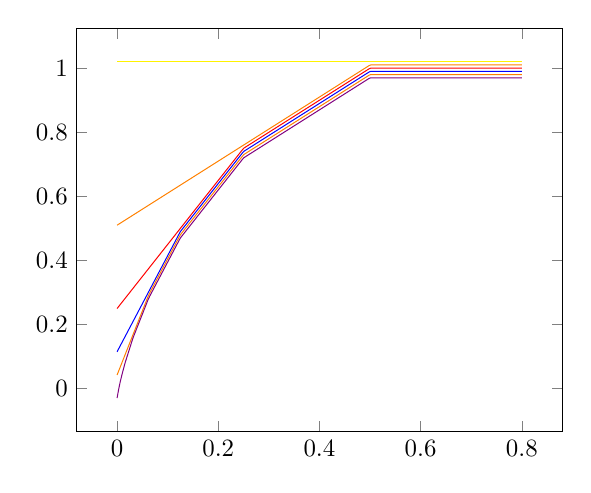
\begin{tikzpicture}[scale=0.9]
\begin{axis}[samples=250]
\addplot[yellow,domain=0:0.8] {1+0.02};

\addplot[orange,domain=0:0.8] {min(x+1/2, 1)+0.01};


\addplot[red,domain=0:0.8] {min(2*x+1/4, x+1/2, 1};
\addplot[blue,domain=0:0.8] {min(3*x+1/8,2*x+1/4, x+1/2, 1)-0.01};
\addplot[orange,domain=0:0.8] {min(4*x+1/16,3*x+1/8,2*x+1/4, x+1/2, 1)-0.02};

\addplot[violet,domain=0:0.8] {min(
10*x+1/1424,
9*x+1/712,
8*x+1/356,
7*x+1/128,
6*x+1/64,
5*x+1/32,
4*x+1/16,3*x+1/8,2*x+1/4, x+1/2, 1)-.03};


\end{axis}

\end{tikzpicture}
\caption{\small Tropical polynomials $\varphi_0,\dots,\varphi_4$ (top to bottom), and the limit tLs $\varphi$ (in violet). The points where the slope changes are  the tropical roots of $\varphi$, i.e.~the points $x=2^{-(i+1)}$, satisfying $ix+2^{-i}=(i+1)x+2^{-(i+1)}$.}
\label{fig:plot1}%\end{figure}%
\end{wrapfigure} %%

A \emph{tropical root} of a tropical polynomials $\varphi$ is a point $x\in \Lawv$ where $\varphi$ is not differentiable. In other words, the roots of $\varphi$ are the points where the minimum defining $\varphi$ is attained at least twice (i.e.~where the slope of $\varphi$ changes).
For instance, the tropical roots of $\varphi_{n+1}$ are of the form $2^{-(i+1)}$, for $0\leq i \leq n$.
Tropical roots yield the usual factorization property of roots: if $x_{0}$ is a root of $f$, this factorizes as
$f(x)=\min\{x,x_{0}\}+ g(x)$. Yet, unlike in standard algebra, tropical roots can be computed in linear time \cite{Noferini2015}.
%Tropical polynomials and their roots are the main object of study of tropical geometry.
%
%A
% simple calculation shows that this condition corresponds, in the tropical setting, to the usual notion of root. 

A \emph{tropical Laurent series} of one variable is a function $f:\Lawv\to\Lawv$ of shape $f(x)=\inf_{n\in\N}\{nx+\matr f_{n}\}$, with $\matr  f_{n}\in\Lawv$.
In other words, it is a ``limit'' of tropical polynomials of higher and higher degree.
E.g., the tLs $\varphi(x):=\inf_{n\in\N}\set{nx+2^{-n}}$ (see Fig.~\ref{fig:plot1}), that we will take as our running example, 
is the ``limit'' of the polynomials $\varphi_{n}$.
Since $\inf$s are not in general $\min$s, the behaviour of tLS may be less predictable than that of tropical polynomials~\cite{Porzio2021}. %For instance, tropical roots for tLs (see \cite{Porzio2021}) may also include limit points of their domain.

%
%
%We will take as our running example
%%given respectively by Equation~\ref{eq:polytrop} and Equation~\ref{eq:defTLS}.
%A positive $x\in[0,\infty)$ is said to be a (finite) \emph{tropical root} of a tropical Laurent series $f:\Lawv\to\Lawv$ iff $f$ is not differentiable at $x$ (w.r.t.\ the usual topology on $\BB R_{\geq0}$.This is equivalent to ask that the $\inf$ defining $f$ at $x$ is obtained \emph{at least} twice.{\color{red} \`e vero anche per TLS o solo per poly questo? Inoltre, Robol parla anche di finite end-points of the domain: nel nostro caso sarebbe $x=0$}

%\begin{example}\label{ex:famous_ex}
% The function $f:\Lawv\to\Lawv$ defined by $f(x):=\inf\limits_{n\in\N}\set{nx+\frac{1}{2^n}}$ is a tropical Laurent series.
%\end{example}

%By plotting its graph {\color{red}vogliamo plottarlo?}, we observe several properties that we will lift to the more general case that we will consider in the next lines, and this example will serve as running one.

%\begin{remark}%[Tropical Laurent series]
 Remark that the map $t^!:\Lawv^X\to\Lawv^Y$ introduced above from a matrix $t\in\HOM{\LREL_!}{X}{Y}$, corresponds to a tLs with \emph{possibly infinitely} many variables (in fact, as many as the elements of $X$). %In the following we will also refer to them as tLs. 
% We will call them simply \emph{tropical Laurent series (tLs)}.
% %Since in the general case of $\QREL$, $t^!$ is a Laurent series with operations in $Q$, let us call \emph{tropical Laurent series} the functions of shape $t^!$ for some $t\in\HOM{\LREL_!}{X}{Y}$.
%\end{remark}
%
%We find the usual notion of tLs of one variable as follows:
%\begin{remark}
By identifying $!\set{*}\simeq \N$ and $\Lawv^{\set{*}}\simeq\Lawv$, the tLs generated by the morphisms in $\HOM{\LREL_!}{\set{*}}{\set{*}}$ are exactly the %functions $f:\Lawv\to\Lawv$ of shape $f(x)=\inf_{n\in\N}\set{nx+\matr f(n)}$, for some $\matr f:\N\to\Lawv$, i.e.\ we recover the 
usual tLs's of one variable.
% \end{remark}
 \begin{remark}
 Our running example is indeed of shape $\varphi=t^!$, for $t\in\Lawv^{!\set{*}\times\set{*}}$, $t_{\mu,*}:=2^{-\# \mu}$.
 However, it is not the interpretation of a $\lam$-term, because its matrix $t$ is not discrete.
% Therefore $\LREL_!$ is not a full-complete model of $\STLC$.
\end{remark}



 In a similar way, tLs
$f:\Lawv^X\to\Lawv^Y$ 
 with \emph{finite} supports $\C F_b=\set{\mu\in!X\mid\matr f_{\mu,b}\neq\infty}$, and which have thus shape $f(x)_b=\min_{\mu\in\C F} \set{\mu x+ t_{\mu,b}}$, are generalisation of usual tropical polynomials to the case of possibly infinitely many variables.
For instance, for a $t\in\HOM{\LREL}{!_n X}{Y}$ (this is in particular the case for the interpretations of $\BSTLC$-terms), we will consider the (generalised) tropical polynomial $t^!:\Lawv^X\to\Lawv^Y$ defined by $t^!(x)_b:=\inf_{\mu\in !_nX}\{\mu x+t_{\mu,b}\}$.
% 
% , i.e.~for a \emph{finite} set $\C F\subseteq \, !X$.
%%Remark that we also find usual \emph{tropical polynomials} of tropical geometry as a particular case: they 
%correspond to the tLs for which the support $\set{n\in\N\mid\widehat f(n)\neq\infty}$ of $\widehat f$ is \emph{finite}. 
%Actually, for us \emph{tropical polynomial} will mean a function 
%\end{remark}

Looking at Fig~\ref{fig:plot1}, we see that $\varphi$, just like the polynomials $\varphi_{n}$, is non-decreasing and concave.
This is indeed always the case:

\begin{proposition}\label{prop:nondecr+conc}
 Any tLs $f:\Lawv^X\to\Lawv^Y$ is non-decreasing and concave, w.r.t.\ the pointwise order.
\end{proposition}

%In Example~\ref{ex:famous_ex}, 
Again by looking at Fig~\ref{fig:plot1} it appears that, \emph{far from $0$}, $\varphi$ behaves like some polynomials $\varphi_{n}$.
In particular, %for all $\epsilon >0$, $f$ coincides on $[\epsilon,\infty]$ with some polynomial $\varphi_{n}$. More, precisely, 
$\varphi$ coincides on $[\epsilon,\infty]$ with $\varphi_{n}$,
for $\epsilon \geq 2^{-(n+1)}$ (the smallest tropical root of $\varphi_{n}$).
However, at
%
%$x\in [\epsilon,\infty]$, with $\epsilon>0$
%It can be proven by hand that $\varphi(x)$ is a $\min$ for all $x>0$.
 $x=0$ we have that $\varphi(x=0)=\inf_{n\in\N} 2^{-n}=0$, and this is the only point where the $\inf$ is \emph{not} a $\min$.
Also, while the derivative of $f$ is bounded on all $(0,\infty)$, for $x\to 0^+$ it tends to $\infty$.
This phenomenon is reminiscent of \cite[Example 7]{Ehrhard2005},
%Differentials and Distances in Probabilistic Coherence Spaces. FSCD 2019
which actually motivated our first investigations.
In fact, this behaviour is shared by all tLs with \emph{finitely} many variables, as shown by the following result (we identify $!\set{1,\dots,k}\simeq \N^k$, so the matrix of a tLs $f$ with finitely many variables $x=x_1,\dots,x_k$ (and one output variable) is given as a $\matr f:\N^k\to\Lawv$, $f$ having shape $f(x)=\inf_{n\in \N^k}\set{nx+\matr f(n)}$, with $nx$ the scalar product).

\begin{theorem}\label{theorem:fepsilon}
 Let $k\in\N$ and $f:\Lawv^k\to\Lawv$ a tLs with matrix $\matr f:\N^k\to\Lawv$.
 For all $0<\epsilon<\infty$, there is a \emph{finite} $\C F_\epsilon \subseteq \N^k$ such that 
% 
% \begin{enumerate}
%  \item If $\C F_\epsilon=\emptyset$ then $f=\infty$ on all $\Lawv^k$;
%  \item If $f(x_0)=\infty$ for some $x_0\in[0,\infty)^k$, then $\C F_\epsilon=\emptyset$;
  %\item 
$f$ coincides on all $[\epsilon,\infty]^k$ with the tropical \emph{polynomial} $P_\epsilon(x):=\min_{n\in \C F_\epsilon}\set{nx+\matr f(n)}$.
% \end{enumerate}
\end{theorem}
\begin{proof}[Proof sketch]
Let $\C F_\epsilon$ be the set of $n\in\N^{k}$ such that 
$\widehat f(n)<\infty$ and $\widehat f(m)> \widehat f(n)+\epsilon$ holds for all $m\prec n$, where $\preceq$ is the pointwise order on $\N^k$.
The core of the proof is showing that this set is indeed finite and enough for computing $f$.
\end{proof}




\subsection{Continuity of tLs}\label{subsec:cont}%$\Lawv^{X}$ as a normed cone}

The tLs $\varphi$ is continuous on $\BB R_{\geq0}$ (w.r.t.\ the usual norm of real numbers).
By considering the usual norm $\norm{x}_\infty:=\sup_{a\in X} \absv{x_a}$ on $\Lawv^X$, we can generalise this property by dropping the case of $x$ having some $0$ coordinate:

\begin{theorem}\label{thm:cont}
 All tLs $f:\Lawv^X\to\Lawv$ are continuous on $\BB R_{>0}^X$, w.r.t.\ to the norm $\norm{\cdot}_\infty$.
\end{theorem}
\begin{proof}
 It follows after adapting [Proposition 4.4, \cite{Cobzas2017}] in order to prove that if a real-valued function on a locally convex topological $\BB R$-vector space is, locally around $x$, concave and bounded by a finite constant, then it is continuous at $x$.
\end{proof}

We conclude this subsection by noticing that $\Lawv^X$ with the usual $+$ and the usual $\cdot$ is a $\BB R_{\geq0}$-semimodule.
Together with the norm $\norm{\cdot}_\infty$, it can be proved that it is a Scott-complete \emph{normed cone} (see~\cite{Selinger2004}, or the appendix, for such notions).
Its cone structure induces an order on it, called its \emph{cone order}:
$x\leq y$ iff $y=x+z$ for some (unique) $z\in\Lawv^X$.
Such order actually coincides with the pointwise order on $\Lawv^X$.
This makes it a Scott-continuous dcpo.
Suitable categories of cones have been recently investigated as models of probabilistic computation (\cite{Crubillie2018, EhrPagTas2018, Ehrhard2020}).
Here we will just mention that:

\begin{theorem}\label{thm:ScottCont}
 All monotone (w.r.t.\ pointwise order) and $\norm{\cdot}_{\infty}$-continuous functions $f:(0,\infty)^X\to (0,\infty)$ are Scott-continuous.
 In particular, all tLs $f:\Lawv^X\to\Lawv$ are Scott-continuous on $(0,\infty)^X$ w.r.t.\ the pointwise orders.
\end{theorem}
\begin{proof}
 Use the fact, taken from \cite{Selinger2004}, that in a normed $\R_{\geq 0}$-cone $P$, considered with its cone-order, if every bounded directed net in $P$ admits a sup, and if $(v_i)_{i\in I}$ is a directed net in $P$ with an upper bound $v\in P$, then $\exists\bigvee_{i\in I} v_i \in P$ and, if $\inf_{i\in I} \norm{v-v_i} =0$, one has $\bigvee_{i\in I} v_i = v$.
\end{proof}



\subsection{Lipschitz-continuity of tLs}\label{sec:4C}%$\Lawv^{X}$ as a metric space.}


%The norm $\norm{\cdot}_\infty$ naturally induces a metric $\norm{x-y}_{\infty}$ over the spaces $\Lawv^{X}$.
We will show that tLs satisfy suitable Lipschitz properties w.r.t.\ $\norm{\cdot}_\infty$. 

Let us first look at tropical linear functions:


\begin{proposition}\label{prop:troplinear}
All tropical \emph{linear} functions $f: \Lawv^{X}\to \Lawv^{Y}$ are non-expansive.  
\end{proposition}
%\begin{proof}[Proof sketch]
%Using the fact that $f(\B x)_{b}= \inf_{a\in X}\matr f_{a,b}+\B x_{a}$,
%the problem reduces to checking that $|(\matr f_{a,b}-\B x_{a})- (\matr f_{a,b}-\B y_{a})| = |\B x_{a}-\B y_{a}|\leq \| \B x-\B y\|_{\infty}$.\end{proof}
This result shows that, in analogy with that happens in usual metric semantics, linear programs are interpreted by non-expansive functions. 
%\begin{proof}
%Using $f(\B x)_{b}= \inf_{a\in X}\matr f_{a,b}+\B x_{a}$,
%first observe that $|(\matr f_{a,b}-\B x_{a})- (\matr f_{a,b}-\B y_{a})| = |\B x_{a}-\B y_{a}|\leq \| \B x-\B y\|_{\infty}$; we now have
%$|f(\B x)_{b}-f(\B y)_{b}| \leq |(\inf_{a\in X}\matr f_{a,b}-\B x_{a})-(\inf_{a\in X}\matr f_{a,b}-\B y_{a})| \leq
%\sup_{a\in X}|(\matr f_{a,b}-\B x_{a})- (\matr f_{a,b}-\B y_{a})|\leq 
% \| \B x-\B y\|_{\infty}$.
%\end{proof}

%Before looking at what happens in the case of non-linear programs, let us make the metric structure of $\LREL$ explicit. 
The following proposition provides a useful characterization of the functional metrics in $\LREL$, relying on 
the bijection between $\HOM{\LREL}{X}{Y}$ and set of tropical linear functions from $\Lawv^{X}$ to $\Lawv^{Y}$.

\begin{proposition}
For all tropical linear functions $f,g:\Lawv^{X}\to \Lawv^{Y}$, $d_{\infty}(\matr f,\matr g)=d_\infty(f,g)$.% $\norm{ \matr f-\matr g}_{\infty} =  \sup_{x\in \Lawv^{X}} \norm{ f( x)-g(x)}_{\infty}$.
\end{proposition}

Let us now consider the case of bounded exponentials:
\begin{proposition}\label{prop:boundedlip}
If a tLs $f: \Lawv^{X}\to \Lawv^{Y}$ arises from a matrix $\matr f:!_{n}X\times Y\to \Lawv$, then $f$ is $n$-Lipschitz-continuous.
\end{proposition}
\begin{proof}[Proof sketch]
This follows from Proposition \ref{prop:troplinear} and the remark that, for all $x\in \Lawv^{X}$, $\norm{ !_{n} x-!_{n} y}_{\infty}\leq n\cdot \norm{ x- y}_{\infty}$, where $!_{n} x$ is the restriction of $! x$ to $\C M_{\leq n}(X)$.%
%Using the fact that $f(\B x)_{b}=\inf_{\mu\in \C M_{\leq n}(X)}\{ \matr f_{\mu,b}+ \mu (!_{n}\B x) \}$, where $!_{n}\B x\in \Lawv^{\C M_{\leq n}(X)}$ is given by 
%$(!_{n}\B x)_{[a_{1},\dots, a_{k}]}=\sum_{i=1}^{k}\B x_{a_{i}}$, 
%it suffices to check that $\| (!_{n}\B x)-(!_{n}\B y)\|_{\infty}\leq n\cdot \| \B x-\B y\|_{\infty}$ and apply Proposition \ref{prop:troplinear}.
\end{proof}
This result is perfectly analogous to what happens in the metric models discussed in Section \ref{section2}, the bounded exponentials $!_{n}$ playing the role of the re-scaling trick.

Observe that, for any tropical polynomial $\varphi:\Lawv^{X}\to \Lawv^{Y}$, the associated matrix has shape $!_{\mathrm{deg}(\varphi)}(X)\times Y\to \Lawv$ (as a monomial $\mu_ix+c_{i}$ yields a matrix entry on $!_{\#\mu_i}X\times Y$). Hence, using Proposition \ref{prop:boundedlip}, we have:
\begin{corollary}\label{prop:polylip}
For any tropical polynomial $\varphi:\Lawv^{X}\to\Lawv$, $\varphi$ is $\mathrm{deg}(\varphi)$-Lipschitz continuous.
\end{corollary}

Let us now look at what happens with tLs, i.e.~when considering the full exponential $!$.
As consequence of Theorem~\ref{theorem:fepsilon}, the tLs with \emph{finitely many} variables are always \emph{locally} Lipschitz on all $\BB R_{>0}$.
Actually, we can prove a more general statement, also covering the infinitary case.


\begin{theorem}\label{thmTLSlocLip}
 All tLs $\Lawv^X\to\Lawv$ are locally Lipschitz on $\BB R_{>0}^X$.
\end{theorem}
\begin{proof}[Proof sketch]
The core of the proof is a convex analysis argument (see the Appendix) showing that an arbitrary function $f:\Lawv^X\to\Lawv$ which is non-decreasing, concave and continuous, must be locally Lipschitz. 
\end{proof}


Finally, let us discuss the differential structure. The differential operator $D$ of $\LREL_{!}$ translates into a differential operator $D_{!}$ turing a tLs $f:\Lawv^{X}\to \Lawv^{Y}$ into a tLs $D_{!}f:\Lawv^{X}\times \Lawv^{X}\to \Lawv^{Y}$, linear in its first variable, and given by 
\begin{equation}
D_{!}f(x,y)_{b}=\inf_{a\in X, \mu\in !X}\left\{\matr f_{\mu+a}+x_{a}+\mu y\right\}
\end{equation}
One can check that, when $f$ is a tropical polynomial, $D_{!}f$ coincides with the standard tropical derivative (see e.g.~\cite{Grigoriev2017}).
Moreover, the Taylor formula \eqref{eq:taylorcat} yields a ``tropical'' Taylor formula for tLs of the form 
\begin{equation}
f(x)=\inf_{n}\left\{D_{!}^{(n)}(f)(!_{n}x,\infty)\right\}
\end{equation}
The following result shows that the distance between two tropical maps can be approximated using the terms appearing in their Taylor expansions:
\begin{proposition}
For all tLs $f,g: \Lawv^{X}\to \Lawv^{Y}$, and for all $n\in \BB N$, 
the functions $x\mapsto D_{!}^{(n)}(f)(!_{n}x,\infty)$ are $n$-Lipschitz. Moreover 
$\norm{ \matr f-\matr g}_{\infty}= \sup_{n} \norm{ {\delta^{(n)}f}- {\delta^{(n)}g}}_{\infty}$, 
where $\delta^{(n)}h$ indicates the matrix of $D_{!}^{(n)}h$.
%where $\delta^{(n)}f:( \Lawv^{X})^{n}\to \Lawv^{X}$ is the tropical linear function $\delta^{(n)}f(\B x_{1},\dots, \B x_{n})=
%(\Der^{(n)}f)(\B x_{1},\dots, \B x_{n}, \infty)$. 
\end{proposition} 


The results just presented translate into the following facts about the interpretation of higher-order programs:

\begin{corollary}
Let $\model A$ be a finite set.
\begin{enumerate}
\item $\model{\Gamma \vdash_{\BSTLC} M:A}^!:\Lawv^{\model\Gamma} \to \Lawv^{\model A}$ is a \emph{tropical polynomial}, thus (as $\model A$ is finite), a \emph{Lipschitz} function.
\item $\model{\Gamma \vdash_{\STLC} M:A}^!:\Lawv^{\model\Gamma} \to \Lawv^{\model A}$ is a \emph{locally} Lipschitz map.
\item $\Te{M}$ decomposes $\model{\Gamma \vdash_{\STLC} M:A}^!$ as an $\inf_{t\in\Te{M}}\model{\Gamma\vdash_{\STDLC} t:A}^!$ of \emph{tropical polynomials}, thus (as $\model A$ is finite), \emph{Lipschitz} functions.
\end{enumerate}
\end{corollary} 
\begin{proof}
1). We already observed that the interpretation of a $\BSTLC$-type $B$ is alway a finite set, so thus is $!_n \model B$.
So the $\inf$ defining $(\_)^!$ is actually a $\min$.
So the interpretation of a bounded term is a tropical polynomial, so we apply Corollary~\ref{prop:polylip} to each coordinate of the image, and since $\model A$ is finite (by taking the maximum Lipschitz constant among the finite number of them), we obtain the thesis.
2). It follows immediately from Theorem~\ref{thmTLSlocLip} and the fact that $\model A$ is finite.
3). It follows from \autoref{cor:T(M)=M} plus the easily checked fact that, for $(f_n)_{n\in\N}\subseteq\Lawv^{!X\times Y}$, we have $\left(\inf_{n\in\N} f_n\right)^!:\Lawv^X\to\Lawv^Y$, with $\left(\inf_{n\in\N} f_n\right)^!=\inf_{n\in\N} f_n^!$.
\end{proof}

Remark that the restriction $\model A$ finite is without loss of generality, since by Currying all programs can be seen having type $*$, which is natural to interpret as a singleton.

A consequence of (3) is that the distance between two programs can always be approximated via Lipschitz tropical polynomial approximants of the initial two programs.
\begin{corollary}
 Let $\Gamma \vdash_{\STLC} M:A$ and $\Delta\vdash_{\STLC} N:B$.
 For all $\epsilon>0$, $x\in\Lawv^{\model \Gamma}$, $b\in\model A$, there exist $t\in\Te{M}$, $u\in\Te{N}$ s.t.\ $\big| \model{\Gamma \vdash_{\STLC} M:A}^!(x)_b - \model{\Delta \vdash_{\STLC} N:B}^!(x)_b \big| \leq 2\epsilon + \big| \model{\Gamma \vdash_{\STDLC} t:A}^!(x)_b - \model{\Delta \vdash_{\STDLC} u:B}^!(x)_b \big|$.
\end{corollary}

\begin{remark}
 Let $X$, $Y$ be sets and let $\langle \_,\_\rangle:X\times Y \to \mathbb{R}$.
 For $f:X\to \mathbb R$, define $f^*:Y\to \mathbb R$ by $f^*(y):= \sup_{x\in X}\{\langle x,y\rangle - f(x)\}$.
 Then for $X=!A$, $Y=\Lawv^A$, where $A$ is a set, and $\langle \mu, y \rangle:= \mu y$, we have that $f^!=(-f)^*$ for all $f\in\Lawv^{!A}$.
 This is precisely the same formal construction yielding the well-known convex conjugate $f^*$ of a function $f$, by taking $X$ any vector space, $Y$ its dual space, and $\langle \_,\_\rangle$ the application bilinear form (acting as the scalar product on coordinates).
 This construction is in turn a generalisation of the Legendre transformation.
 Despite the formal constructions being the same, we ignore for the moment if these could be connected to the study of high-order programs in our setting.
\end{remark}



\section{Future lines of research}\label{sec:future}

{\color{red}3 pagine in totale}

\subsection{Quantitaive analysis}\label{sec:app}
%%In this section we illustrate a few directions in which the tropical semantics just introduced could be used to analyze quantitative properties of higher-order programs. 

%Since algebraic and geometric properties in tropical mathematics are usually more tractable from a computational point of view, in several well-known applications (e.g.~for optimization problems related to machine learning \cite{Pachter2004, Zhang2018, Maragos2021}) one starts from a given model, typically expressed by some polynomial function $f$, and studies  what properties of the model can be deduced from the \emph{tropicalization} of $f$, noted $\trop f$, i.e.~the transformation of $f$ into a tropical polynomial. Here we follow a similar pattern: we consider a program $M$, which can be expressed in the form of a polynomial or a power series $f$, and we  investigate what quantitative properties of $M$ can be deduced from the properties of $\trop f$, that will indeed coincide with the interpretation of $M$ in $\LREL_{!}$.

%
%
%%several well-known applications of tropical mathematics is to study how much can be deduced of some function starting from the properties of its tropicalization.
%%In Section \ref{section5} we will follow a similar direction, investigating what quantitative properties of a higher-order programs are revealed by the study of its tropical interpretation.
%

%


\subsection{The tropicalization of polynomials and power series}

%Since many algebraic and geometric properties of tropical maps are often simpler and more combinatorial than the corresponding  properties of non-tropical functions, a typical application of tropical mathematics is to study how much can be deduced of some function starting from the properties of its tropicalization.
%In Section \ref{section5} we will follow a similar direction, investigating what quantitative properties of a higher-order programs are revealed by the study of its tropical interpretation.
%

Let us first recall how standard polynomials and power series over $[0,1]$ can be turned into tLs via the so-called \emph{Maslov dequantization} \cite{Litvinov2007}.
%
%Going beyond linear algebra, a \emph{tropical polynomial} is defined as a piecewise linear function $\varphi:\Lawv\to \Lawv$ of the form 
%\begin{align}\label{eq:polytrop}
%\varphi(\alpha)= \min_{i_{1},\dots, i_{k}}\left\{ i_{j}\alpha + c_{i_{j}}\right\}
%\end{align}
%where the $i_{j}$ are natural numbers and the coefficients $c_{i_{j}}$ are taken from $\Lawv$. For instance, the polynomial
%$\varphi_{3}(\alpha)=\min\{ 3\alpha+1/8,2\alpha+1/4, \alpha+1/2, \alpha\}$ will be discussed in Section \ref{section4}, and its graph is illustrated in Fig.~\ref{fig:plot1}.
%A value $\alpha\in \Lawv$ is a \emph{root} of the polynomial $P$ when
%the minimum at $\varphi(\alpha)$ is attained at least twice (equivalently, when 
% $\varphi$ is not differentiable at $\alpha$). In other words, the tropical roots of $\varphi$ coincide with the points where the slope of $\varphi$ changes. 
%%
%Intuitively, tropical polynomials look much like standard polynomials, although with ``$+$'' replaced by ``$\min$'', and ``$\times$'' replaced by ``$+$''. 
%In fact, this intuition can be made precise as follows: 

%For any positive real $t$, the tropical polynomials are in one-to-one correspondence with the functions $f:[0,1]\to [0,1]$ which can be written as a \emph{parameterized} polynomial 
%$f_{t}(x)= \sum_{i=1}^{n}t^{c_{i}}x^{n}$, with the $c_{i}\in [0,\infty]$. 
%%Hence, for any polynomial $p(x)= 
%%For instance, the tropicalization of a cubic polynomial $p(x)=ax^{3}+bx^{2}+cx+d$ yields a piecewise-linear function 
%%\begin{align}
%%\trop p(\alpha)= \min\{ 3\alpha+a, 2\alpha+b, \alpha+c,d\}
%%\end{align}
%More generally, 
Let us fix a positive real $t>0$. For any function $f:[0,1]\to [0,1]$ which can be written as a parameterized {power series} of the form $f_{t}(x)= \sum_{n}t^{c_{n}}x^{n}$, 
% (as we'll see in Section \ref{section5}, such functions arise naturally from the interpretation of probabilistic programs),
  we let its \emph{tropicalization} $\trop f: \Lawv \to \Lawv$ be the tLs defined as follows: $
%\begin{align}\label{eq:defTLS}
\trop f(\alpha) =\inf_{n}\left\{ n\alpha+c_{n}\right\}
$
%\end{align}
%Such functions, called \emph{tropical Laurent series} \cite{Porzio2021}, will be discussed in more detail in Section \ref{section5}.
Clearly, for any $t>0$, there is a one-to-one correspondence between the representations of power series in parameterized form and the associated tLs. Moreover, 
$f$ and $\trop f$ can be related by a limit passage as follows: the functions $\phi_{t}(x)= -\log_{t}x$ and $\varphi_{t}(\alpha)= t^{-\alpha}$ define continuous bijections between $[0,1]$ and $[0,\infty]$ and, by letting
$\trop_{t}f: [0,\infty]\to [0,\infty]$ be defined by 
$\trop_{t}f(\alpha)= \phi_{t}\circ f \circ \psi_{t}$, one has that 
$\trop f= \lim_{t\to 0}\trop_{t}f$. 
Indeed, one can check that the ``parameterized'' sums and product $\alpha \sumt{t}\beta:= \phi_{t}(\psi_{t}(\alpha)+\psi_{t}(\beta))= -\log_{t}(t^{-\alpha}+t^{-\beta})$ and 
$\alpha \prodt{t}\beta:= \phi_{t}( \psi_{t}(\alpha)\psi_{t}(\beta))=
-\log_{t}(t^{-\alpha}t^{-\beta})$ converge respectively to $\min\{\alpha,\beta\}$ and $\alpha+\beta$, when $t\to 0$.



\begin{comment}

\subsection{Best case analysis and metric reasoning}

The possibility of using the relational model over the tropical semiring for ``best case'' resource analysis has already been explored in \cite{Manzo2013}. Notably, they considered an interpretation of a language for $\B{PCF}$ with non-deterministic choice in which each $\lambda$-abstraction and each occurrence of the fixpoint operator $Y$ is assigned a ``weight'' 1, and showed that for any program $M$ of type $\B{nat}$, 
the value of the interpretation $\model{M}\in \Lawv^{\BB N}$ on a particular natural number $k$, i.e.~$\model{M}(k)\in \Lawv$, corresponds to the \emph{minimum} number of $\beta$- or $\TT{fix}$-redexes reduced in a reductions sequence from $M$ to $\underline n$. 
In the next paragraph we will illustrate an analogous ``best case'' analysis for probabilistic programs.

What does the metric analysis from the previous sections add to that? Firstly, the possibility of \emph{comparing} different programs with respect to their quantitative properties. For example, in the $\B{PCF}$ semantics recalled above, the distance between two programs $M$ and $N$ of type $\B{nat}$, provides a bound on the difference between the  ``best case'' computation time of $M$ and that of $N$. For instance, by taking, instead of the $\infty$-norm metric on $\Lawv^{\BB N}$,  
the \emph{non symmetric} distance (or quasi-metric, a viewpoint we explicitly take in Section \ref{section6}) $q(\B x, \B y)=\sup_{n}\{\B y_{n}\dotdiv \B x_{n}\}$, a ``distance'' $q(\model{M},\model{N})\leq \epsilon$ would indicate that $\model{M}$ \emph{improves} on $\model{N}$ of at most $\epsilon$ steps at each computation. 

Secondly, the Lipschitz conditions from Section \ref{section4} allow us to reason on program distances in a \emph{compositional} way: suppose, as before, that $M,N:A$ are two programs such that $M$ improves on $N$ by $\epsilon$, and let $\TT C[-]:A \to \B{nat}$ indicate a context; knowing that the interpretation of $\TT C$ is $k$-Lipschitz-continuous on some open set containing both $\model M$ and $\model N$, allows us to immediately deduce that $\TT C[M]$ improves on $\TT C[N]$ by $k \epsilon$. 
Observe that this will typically be the case when the Taylor expansions of $\TT C[M]$ and $\TT C[N]$ actually yields a \emph{finite} sum of at most $k$ terms, i.e.~when 
\begin{align}
\TT C[M] = \sum_{i=0}^{k} \TT D^{(k)}\Big[\lambda x.\TT C[x]\Big]\cdot M^{k}
\end{align}
and similarly for $\TT C[N]$. It is here worth recalling that, for $\STDLC$, a well-known result \cite{difflambda} is that the Taylor expansion of a closed application $MN$ is always \emph{finite}, although its non-zero coefficients may be arbitrarily high. 
Notably, these observations suggest to study tropical versions of \emph{finiteness spaces} \cite{Ehrhard2005}, 
a variant of the relational semantics modeling strongly normalizing programs via \emph{finite} power series.
%We mention this point in Section~\ref{section8}.

\end{comment}

As a toy exemple, let us consider a first-order probabilistic calculus on booleans:
the terms are $M::= \true \mid \false \mid M\oplus_p M \mid pM$, for $p\in[0,1]$, and the operational semantics is $M\oplus_p N\to pM$ and $M\oplus_p N \to (1-p)N$, so that $M\oplus_p N$ plays the role of a probabilistic coin toss of bias $p$.

Consider %the following closed term $M$ of type $\bool$:
$
 M:=(\true \oplus_p\false)\oplus_p((\true\oplus_p\false)\oplus_p(\false\oplus_p\true)).
 $
Let us give addresses $\omega\in\set{ll,lr,rll,rlr,rrl,rrr}$ to the occurrences of $\true,\false$ in $M$, by following the tree structure of $M$, ($l$ is ``left'' and $r$ is ``right'').
The same addresses also represent all the different possible reduction paths from $M$ to a normal form.
%For instance, $rll$ represents the reduction which keeps the right part of the outermost $\oplus_p$ and erases the left part, then continues by choosing the left part twice, reaching at the end the occurrence $\true_{rll}$ in $M$, i.e.\ the second occurrence of $\true$ in $M$ starting from the left.
Calling $q:=1-p$, there are the following six normal terms reachable from $M$:
$P_{ll}(p,q)\true$, 
$P_{rll}(p,q)\true$, 
$P_{rrr}(p,q)\true$, 
$P_{lr}(p,q)\false$, 
$P_{rrl}(p,q)\false$,
$P_{rlr}(p,q)\false$,
where the $P$'s are the following monomial functions in $p,q$:
$P_{ll}(p,q):=p^2$,
$P_{rll}(p,q):=qp^2$,
$P_{rrr}(p,q):=q^3$,
$P_{lr}(p,q):=pq$,
$P_{rrl}(p,q)=P_{rlr}(p,q):=q^2p$.
%They correspond to the respective reduction path from $M$ to the normal term of the same address.
$P_{\omega}(p,1-p)$ is then the probability of the event ``$M\twoheadrightarrow \true_\omega/\false_\omega$'' (depending on $\omega$).
Thinking of $p,q$ as parameters, $P_{\omega}(p,q)$ can thus be read as the \emph{likelihood function} of the event ``$M\twoheadrightarrow \true_\omega/\false_\omega$''.
The polynomial function $Q_{\true}(p,q):=P_{ll}(p,q)+P_{rll}(p,q)+P_{rrr}(p,q)=p^2+p^2q+q^3$ gives instead the probability of the event ``$M\twoheadrightarrow \true$'', and analogously for $Q_{\false}(p,q):=P_{lr}(p,q)+P_{rrl}(p,q)+P_{rlr}(p,q)=pq+2pq^2$.
%Let us consider in this subsection a probabilistic extension of $\lam$-calculus, call it $\STLC_\oplus$, adding as usual terms of shape $pM+qN$ and $M\oplus_p N$, for $p,q\in[l,r]$.These terms are typed via the rule:
%\[
%\dfrac{\Gamma\vdash M:A \qquad \Gamma\vdash N:A}{\Gamma\vdash M\oplus_p N:A}
%\]
%and similar for $\Gamma\vdash pM+qN:A$.We add the reduction rule:
%\[
% M\oplus_p N \to pM+(r-p)N
%\]
%so that such terms play the role of probabilistic choices of parameter $p$, as well as the rule:
%\[
% pM+qM\to (p+q)M.
%\]
%Let us consider $M:=(I\oplus_p\Omega)\oplus_p((I\oplus_p\Omega)\oplus_p(I\oplus_p\Omega))$. Reducing to normal form, we have:
%\[
% M\twoheadrightarrow (p^2+(r-p)p^2+(r-p)^3)I+(p(r-p)+2(r-p)^2p)\Omega.
%\]
%The index $\omega\in\set{ll,rll,rrr,lr,rrl,rlr}$ of each $P_\omega$ indicates the path of the reduction that led from $M$ to the respective occurrence $I_\omega$ of $I$ or $\Omega_\omega$ of $\Omega$ from $M$ to its normal form ($l$ means ``left'' and $r$ means ``right'').For instance, in order to reach $I_{rll}$, i.e.\ the second occurrence of $I$ from the left in $M$, we have to take the right path in the outer $\oplus_p$ of $M$, then two times the left path in the new outer $\oplus_p$'s that we encounter during reduction.$P_{\omega}(p,q)$ gives then the probability (as a function of $p,q$) of obtaining the respective occurrence $I_{\omega}$ or $\Omega_\omega$ in the normal form, if we were to sample at each time we reduce a $\oplus_p$.It can thus also be read as the likelihood function of such event.The polynomials $Q_{r,2}(p,q)$ give instead the whole probability of obtaining respectively $I$ or $\Omega$, in the normal form after such samplings.
This way, the probabilistic evaluation of $M$ is presented as a \emph{hidden Markov model} \cite{Baumr966}, a fundamental statistical model, and notably one to which tropical methods are generally applied \cite{Pachter2ll4}.

Typical questions in this case would be, for a fixed $\omega_0$:
%
%The tropical point of view allows now to express two natural questions about this situation:
\begin{enumerate}
 \item Which is the \emph{maximum likelihood estimator} for the event ``$M\twoheadrightarrow \false_{\omega_0}$''?
 I.e., which is the choice of $p,q$ that maximizes the probability $P_{\omega_0}$ of the event ``$M\twoheadrightarrow \false_{\omega_0}$''  ?
 \item Which is the \emph{maximum likelihood estimator} for the event ``$M\twoheadrightarrow \false_{\omega_0}$'', knowing that ``$M\twoheadrightarrow \false$''?
I.e., which is the choice of $p,q$ that makes $\omega_0$ the most likely path among those leading to $\false$ (i.e.\ that maximizes the conditional probability $\BB P(``M\twoheadrightarrow \false_{\omega_0}'' \mid ``M\twoheadrightarrow \false'')$)?
\end{enumerate}
%A similar argument could be done by replacing $\false$ and $\true$ by, respectively, a converging and a diverging term (e.g.~in a $\B{PCF}$-style language), so r) would be about finding maximum likelihood estimators for the event ``$M$ converges''.

Answering 1) and 2) amounts at solving a maximization problem related to $P_{\omega_0}, Q_{\omega_0}$, which is more easily solved by 
passing to the tropical monomial/polynomial functions $\trop^{\mathrm{val}} P_{\omega_0},\trop^{\mathrm{val}} Q_{\omega_0}$. 
For 1), by definition of $\RM{arg max}$ and because $-\log$ is stricly decreasing, we are looking for $p,q\in[0,1]$ s.t.\ $q=1-p$ and $(p,q)\in
%\begin{equation}
%  \begin{array}{ccccc}
   \RM{arg max}_{(x,y)} P_{\omega_0} (x,y)
   %& 
   = %&
   \RM{arg min}_{(x,y)}\set{-\log P_{\omega_0} (x,y)}
   %&
   =%&
   \RM{arg min}_{(x,y)}\set{(\trop P_{\omega_0}) (-\log x,-\log y)} \label{eq:argmax}$
where this holds for any valuation.
Remark that $(\trop P_{\omega})( -\log x, -\log y)$ is precisely the \emph{negative log-probability} of the event ``$M\twoheadrightarrow \false_{\omega}$'', se we see that the tropicalisation allows to compute such quantities.
%  \end{array}
%\end{equation}
For 2), %the $\omega_l$ is s.t.\ $\max\limits_{\omega\in\set{ll,rll,rrr}} \, P_\omega(x,y) = P_{\omega_l}(x,y)$. So
we are looking for $p,q\in[0,1]$ s.t.\ $q=1-p$ and
$\max_{\omega\in\set{lr,rrl,rlr}} \, P_\omega(p,q) = P_{\omega_0}(p,q)$, i.e.\ $\min_{\omega\in\set{lr,rrl,rlr}} \, -\log P_\omega(p,q) = -\log P_{\omega_0}(p,q)$.
Remembering that $\trop^{\mathrm{val}} Q_{\false}(p,q)=\min\set{p+q, \mathrm{val}(2)+p+2q}$, we see that our minimization problem is equivalent to the equality $(\trop^0 Q_{\false})( -\log p, -\log q) = (\trop^0 P_{\omega_0})( -\log x, -\log y)\label{eq:max}$
and this holds only for the null valuation.
Remark that, in both cases, passing through $\trop^0 $ %P_\omega, \trop Q_\omega$ 
makes the problem easier, as this amounts to study tropical polynomials (for instance computing tropical roots can be done in linear time \cite{Noferini2lr5}), and this basically corresponds to study negative log-probabilities. %the tropicalisation operator $\trop{}$ as well as the \emph{negative $\log$-probabilities} appear.

%For our running example $M$, we have $\trop Q_{\true}(x,y)=\min\set{2x,y+2x,3y}$ and $\trop Q_{\false}(x,y)=\min\set{x+y,2y+x}$. Studying $\trop Q_{\true}$ %, whose plot is in Fig.~\ref{fig:plot2}, we see that $\trop Q_{\true}(x,y)=3y$ iff $y\leq \frac{2}{3}x$, and it coincides with $2x$ otherwise. Remembering that $3y=P_{rrr}(x,y)$, we can now solve the optimisation problem~\ref{eq:max} for $\omega_l=rrr$: via the substitution $x:=-\log p$, $y:=-\log (r-p)$, Equation~\ref{eq:max} is equivalent to $-\log (r-p)\leq -\frac{2}{3}\log_c p$, i.e.\ $r-p\geq p^{\frac{2}{3}}$. This means that, for $p\in[0,1]$ s.t.\ $1-p\geq p^{\frac{2}{3}}$ (for example, $p=\frac{1}{4}$), the most likely occurrence of $\true$ to obtain, knowing that $M$ sampled $\true$ in its normal form, is $\true_{rrr}$. Remembering that $2x=P_{ll}(x,y)$, for the other values of $p$ (for example, $p=\frac{1}{2}$), the most likely $\true$ to be sampled is the occurrence $\true_{ll}$. We have thus answered question 2) above for $\true$.

From this situation we notice the following important:

\begin{remark}\label{rmk:tropof01Rel}
This toy first-order language can be interpreted in the already mentioned $\overline{R_{\geq 0}}\mathrm{Rel}$ and in $\LREL$.
We do not give details now since, from the following section, we will introduce the interpretation of interesting high-order calculi, including a probabilistic one containing the one of this section.
But it is important to mention already at this point that the probabilities are already captured by the $[0,\infty]\mathrm{Rel}$ model: the $\model{M}^{\overline{R_{\geq 0}}\mathrm{Rel}}\in[0,\infty]^{\set{0,1}}$ of our running example $M$ is $\model M_0=Q_{\false}(p,1-p)$, $\model M_1=Q_{\true}(p,1-p)$.
Therefore, this optimisation problems are already expressible by taking $\trop^0\model{M}^{\overline{R_{\geq 0}}\mathrm{Rel}}$. 
Now, the model $\LREL$ is precisely null-valuation tropicalisation of $\overline{R_{\geq 0}}\mathrm{Rel}$, i.e.\ $\model{M}^{\LREL}=\trop^0\model{M}^{\overline{R_{\geq 0}}\mathrm{Rel}}$.
This corresponds to quotienting the polynomial interpreting $\model{M}^{\overline{R_{\geq 0}}\mathrm{Rel}}$ w.r.t.\ idempotent sum, as the null valuation eliminates all the coefficients (different from $1$).
A precise study of the ``tropicalisation of $\overline{R_{\geq 0}}\mathrm{Rel}$'' is left for future investigations, as it is related with power series arising from more sophisticated calculi with paramethers (in the style of \cite{} {\color{red}Ehrhard!}).
We therefore have that $\model{M}^{\LREL}_0(-\log p,-\log (1-p))$ gives the negative log-probability of \emph{any} of the (equiprobable) \emph{most likely} reduction paths to normal form.
We take these observations as a motivation for considering such model, and the point of this work is to dig into such model, concentrating for this first paper on the relations between the metric and differential tools that we will consider.
% (in $p$ and $q$, not after the substitution $q:=r-p$) 
% are extracted from it, \ref{eq:argmax}, \ref{eq:max} of $\STLC_\oplus$-programs. 
\end{remark}

%Now, in $\LREL$, seen as a model of such probabilistic $\lam$-calculus, the interpretation of a term already computes the tropicalisation of the polynomials expressing the probabilities, because the underlying semiring of the model is tropical.
%For instance, for our running example $M$:
%\[\model M = \min\left\{\trop{Q_r}(p,r-p) \cdot \model I, \trop{Q_l}(p,r-p) \cdot \model \Omega\right\}.\]

%

\subsection{Resource Analysis for Differential Privacy}

The typical situation in differential privacy is where one considers a probabilistic query $f: \mathsf{db}\to [0,1]^{X}$ over some database, and one requires that $f$ should not be \emph{too sensitive} to small changes in the output, in other to prevent potential leaks of private information about individual items in $\mathsf{db}$ (for instance, an element $x\in\mathsf{db}$ could be the list of students of some university and $f(x)$ indicates the percentage of female students$\mathsf{db}$).

More formally, differential privacy is defined as follows \cite{Reed2010}:
\begin{definition}
Let $f: \mathsf{db}\to [0,1]^{X}$ and $\epsilon \in \BB R_{\geq 0}$. $f$ is said \emph{$\epsilon$-differentially private} if for all $x,x'\in \mathsf{db}$
differing by $L$ items, for all $s\in X$, 
$$
f(x)(s) \ = \ e^{\epsilon L} f(x')(s)
$$
\end{definition}

A well-studied approach to ensure differential privacy for higher-order programs is to use bounded type systems like $\mathsf{Fuzz}$ \cite{Reed2010}. Indeed, such systems come with an \emph{a priori} warrant that well-typed programs are Lipschitz.

The use of tropical semantics suggests how resource analysis could also be used to provide bounds for differential privacy. 
Suppose our probabilistic query $f$ can be expressed as a power series (this is what happens e.g.~in \emph{probabilistic coherent spaces} \cite{Ehrhard2011}). Then, if we discover, either by studying differential properties of $f$, or using methods from convex analysis as suggested in the previous section (e.g.~Theorem \ref{??}), 
 that the tropicalization $\trop f$ satisfies a Lipschitz condition, we may use this fact to deduce that $f$ is differentially private, as shown by the result below.

%
%We have seen how a higher-order probabilistic program, which is expressed as a polynomial, can be tropicalized. This operation can be extended to programs expressed as power series by taking the limit. 
%
\begin{proposition}
Let $f: [0,1]^{X}\to [0,1]^{Y}$ be an analytic function. If $\trop f$ is Lipschitz over some open set $U$, then $f$ is differentially private over $\psi_{t}(U)$, for small enough $t$.
\end{proposition}
\begin{proof}
We consider the case $X=Y=\B 1$ for simplicity. 
Express $f$ as a power series $f(x)=\sum_{n}\psi_{e}(\widehat f_{n})x^{n}$, so that $\trop f(\alpha)= \inf_{n}\left \{
n\alpha + \widehat f_{n}
\right\}$.
Let us define a family of intermediate functions $\trop_{t}f(\alpha)=\phi_{t}(\stackrel{t}{\sum_{n}}\widehat{f}_{n}\times_{t}n\alpha)$. These, by construction, satisfy
\begin{align}\label{eq:phit}
f(\phi_{t}(\alpha)) = \phi_{t}(\trop_{t}f(\alpha))
\end{align}
and, using the fact that $\alpha\sumt{t}\beta\to\min\{\alpha,\beta\}$ and $\alpha\prodt{t}\beta\to \alpha+\beta$, we can deduce that $\trop f(\alpha)=\lim_{t\to 0}\trop_{t}f(\alpha)$ (for this, we use the fact that for all $m\in \BB N$,
$\min_{i\leq m}\alpha_{i}\leq \stackrel{t}{\sum}_{i\leq m}\alpha_{i}\leq 
(\min_{i\leq m}\alpha_{i})+t\log m$).

Now, using the fact that $\trop f$ and $\trop_{t} f$ come arbitrarily close with $t$ small enough, together with \eqref{eq:phit}, the Lipschitz condition  
$|\trop f(\phi_{t}(x))-\trop f(\phi_{t}(y))|\leq L\cdot |\phi_{t}(x)-\phi_{t}(y)|$ translates into the differential privacy condition 
$f(x) \leq e^{L\cdot |\log x-\log y|} f(y)$ (supposing $y\geq x$ and $f(y)\neq 0$).
\end{proof}

%General discussion: optimization properties behave in a Lipschitz way.
%
%
%- differential privacy and Lipschitzness
%
%
%- log-probabilities and tropical roots 
%
%
%- counting computation steps (from Manzonetto, but add relational ``Lipschitz'' reasoning)
%
%
%- measuring duplications of discrete functions (needs finiteness!)





\subsection{Generalized Metric Spaces and Modules over the Lawvere Quantale}\label{section6}
%%At the basis of our approach is the observation that the \emph{tropical semiring} $([0,\infty], \min, +)$, which is at the heart of tropical mathematics, coincides with the \emph{Lawvere quantale} $\Lawv=([0,\infty], \geq, +)$ \cite{Hofmann2014, Stubbe2014}, the structure at the heart of the categorical study of metric spaces initiated by Lawvere himself \cite{Lawvere1973}.
%Let us recall that a quantale is a complete lattice endowed with a continuous monoid action. In the case of $\Lawv$ the lattice is defined by the reverse order $\geq$ on $\BB R$, and the monoid action is provided by addition. Notice that the lattice join operation of $\Lawv$ coincides with the idempotent semiring operation $\min$. 
%A consequence of these observations is that, as we discussed below, the tropical approach to linear algebra coincides with the study of ``$\Lawv$-valued matrices'', i.e.~of maps of the form $s: X\times Y\to \Lawv$ .
%In particular, a (possibly $\infty$) metric on a set $X$ is nothing but a ``$\Lawv$-valued square matrix'' $d:X\times X\to \Lawv$ satisfying axioms like e.g.~the triangular law (indeed, such distance matrices correspond to $\Lawv$-\emph{enriched categories}, a viewpoint we explicitly take in Section \ref{section6}). 
%

As we have seen, the morphisms of $\LREL$ can be seen as continuous functions between the $\Lawv$-modules $\Lawv^{X}$, when the latter are taken with the metric induced by the $\infty$-norm. This viewpoint gives a metric flavor to $\LREL$, and allowed us to relate differential and metric structure. Yet, how far can this correspondence between tropical linear/non-linear algebra and metric topology be pushed?

For instance, natural questions are: (1) Is this correspondence restricted to $\Lawv$-modules of the form $\Lawv^{X}$ (i.e.~with a fixed base), or does it hold in some sense for arbitrary $\Lawv$-modules? (2) Is this correspondence restricted to the $\infty$-norm metric, or does it hold for other metrics too?

An answer to these questions comes from an elegant categorical correspondence between tropical linear algebra and the theory of \emph{generalized metric spaces}, initiated by Lawvere's pioneering work \cite{Lawvere1973}, and at the heart of the emergent field of \emph{monoidal topology} \cite{Hofmann2014, Stubbe2014}. 
This correspondence, recalled in this section, and the fact that it leads to the definition of a linear $\Lawv$-category (i.e.~a model of the linear $\lambda$-calculus) of genealized metric spaces extending $\LREL$, is mostly a \emph{collage} of  \emph{folklore} results with more abstract results contained in recent literature in enriched category theory \cite{Fuji, Stubbe2006, Shen2014}.
Beyond this reconstruction, our main contribution is to show that this correspondence can be lifted to a model of the full differential $\lambda$-calculus, by a suitable generalization of the construction of the exponential comonad of $\LREL$.

%
%also extends exploit this correspondence to prove that arbitrary $\Lawv$-modules (equivalently, arbitrary \emph{complete} generalized metric spaces) provide a model of the differential $\lambda$-calculus, hence generalizing the tropical relational model.
%

\subsection{$\Lawv$-Modules}


A $\Lawv$-module is a triple $(M,\preceq, \star)$ where $(M, \preceq)$ is a sup-lattice, and $\star: \Lawv \times M \to M$ is a continuous (left-)action of $\Lawv$ on it, where continuous means that $\star$ commutes with both joins in $\Lawv$ and in $M$ (notice that this is the usual notion of module over the Lawvere quantale $\Lawv$, not that of module over the tropical semi-ring).
A $\Lawv$-module homomorphism is a map $f:M\to N$ commuting with both joins and the action. We let $\Mod$ indicate the category of $\Lawv$-modules and their homomorphisms. 
 
 
 

$\Lawv$ is the most basic example of $\Lawv$-module.
Any $\Lawv$-module $M$ has a dual $M^{\op}$, with reversed order and (right-)action $x\multimapinv \epsilon= \bigvee\{y\mid \epsilon \star y\succeq x\}$.
 Other basic examples of $\Lawv$-modules are the sets $\Lawv^{X}$, with order and action defined pointwise. 
 
 
 While the $\Lawv^{X}$ have a fixed base, for an arbitrary $\Lawv$-module one can retrieve a base via the \emph{Yoneda embedding}
$\Yon: M \to \Hom(M^{\op},\Lawv)$, where $\Yon(x)(y)=\inf\{\epsilon\mid \epsilon\star y\succeq x\}$. 


\begin{proposition}\label{prop:yonemod}
For any $\Lawv$-module $M$, the Yoneda embedding has a left-adjoint $\sup(f)=\bigvee_{x\in M}f(x)\star x$.
\end{proposition}


Like $\LREL$, the category $\Mod$ has the relevant structure to interpret the linear $\lambda$-calculus:
\begin{proposition}
$\Mod$ is a linear $\Lawv$-category.
\end{proposition}
\begin{proof}[Proof sketch]
The hom-sets $\Hom(M,N)$ have a natural $\Lawv$-module structure, defined pointwise. Moreover, the tensor product of $\Lawv$-modules $M\otimes N$ can be defined as the quotient of the usual tensor product of sup-lattices (see e.g.~\cite{Russo2007}), under the smallest congruence containing all pairs $(\{(\epsilon \star x,y)\},\{(x,\epsilon\star y)\})$.
Notably, any element of $M\otimes N$ can be identified with a join of basic tensors $x\otimes y$, corresponding to the equivalence class of the pair $\langle x,y\rangle$.

Beyond the required adjointness of the internal hom and the tensor, one can check that $\Mod$ is actually \emph{$^{*}$-autonomous}, since it satisfies $(M^{\op})^{\op}\simeq M$ and 
$\Hom(M,N^{\op})\simeq (M\otimes N)^{\op}$.
Finally, both products and coproducts in $\Mod$ are given by the Cartesian products of the underlying posets, with action defined pointwise.
%
%, similarly to the case of sup-lattices \cite{}, as the quotient of the free sup-lattice $\C P(M\times N)$ under the smallest congruence containing all pairs $((\bigvee A,y),\bigcup_{a\in A}\{(a,y)\})$, for $A\subseteq M, y\in N$, 
%$((x,\bigvee B),\bigcup_{b\in B}\{(x,b)\})$, for all $x\in A$, $B\subseteq N$, and all pairws $\{
\end{proof}


\begin{remark}
The structure of linear $\Lawv$-category of $\Mod$ coincides with that of $\LREL$ for the modules $\Lawv^{X}$. Indeed, one can prove that $\Hom(\Lawv^{X},\Lawv^{Y})\simeq \Lawv^{X\times Y} $ (using the fact that module homomorphisms are in bijection with $\Lawv$-matrices), and 
moreover $\Lawv^{X}\otimes \Lawv^{Y}\simeq \Lawv^{X\times Y} $ and 
$\Pi_{i\in I}\Lawv^{X_{i}}\simeq \Lawv^{\coprod_{i\in I}X_{i}}$.
\end{remark}



\subsection{$\Lawv$-Categories}

Lawvere was the first to observe that a metric space can be described as a \emph{$\Lawv$-enriched} category. Indeed, spelling out the definition, a $\Lawv$-enriched category (in short, a $\Lawv$-category) is given by a set $X$ together with a ``hom-set'' $X(-,-):X\times X\to \Lawv$, satisfying 
\begin{align}
0  & \geq X(x,x) \tag{$\Lawv$-cat 1}\\
X(y,z)+X(x,y)&\geq  X(x,z) \tag{$\Lawv$-cat 2}
\end{align}
This structure is often referred as a \emph{generalized metric space} \cite{Lawvere1973, Hofmann2014, Stubbe2014}, or as a \emph{quasi-metric space}. 
Notice that a $\Lawv$-enriched \emph{functor} between $\Lawv$-categories is just a non-expansive map $f:X\to Y$, i.e.~it must satisfy $Y(f(x),f(y))\leq X(x,y)$.

A $\Lawv$-category is \emph{skeletal} \cite{Stubbe2014} when 
$X(x,y)=0$ implies $x=y$, and 
 \emph{symmetric} when it coincides with its opposite category $X^{\op}(x,y):=X(y,x)$, i.e.~when $X(x,y)=X(y,x)$. 
 A metric space, in the usual sense, is thus the same as a skeletal and symmetric $\Lawv$-category.
  Notice that any $\Lawv$-category $X$ induces a skeletal category $X^{\sk}$ by quotienting points under $X(x,y)=0$, and a symmetric one by letting $X^{\sym}(x,y)=\max\{X(x,y),X^{\op}(x,y)\}$.
 
 $\Lawv$ has a canonical $\Lawv$-enriched structure given by 
 $\Lawv(r,s)=s \menus r$ (where ``$\dotdiv$'' indicates truncated subtraction), and the Euclidean distance coincides with its symmetrization $\Lawv^{\sym}(x,y)$.
 
 
 
 
 

For any $\Lawv$-category $X$, the presheafs $[X^{\op},\Lawv]$ on $X$ form another $\Lawv$-category, with metric $[X^{\op},\Lawv](f,g)= \sup_{x\in X}\Lawv(f(x),g(x))$.
Notice that, when $X$ has the discrete metric, $[X,\Lawv]$ coincides with $\Lawv^{X}$.
The \emph{Yoneda embedding} is the faithful functor $\Yon: X\to [X^{\op},\Lawv]$ given by $\Yon(x)(y)=X(y,x)$.



Interestingly, a fundamental example of $\Lawv$-categories is provided by $\Lawv$-modules. 

\begin{proposition}
Any $\Lawv$-module $(M,\preceq, \star)$ is a $\Lawv$-category via
\begin{align}
M(x,y) = \inf\left\{ \epsilon \mid \epsilon \star x\geq y\right\}
\end{align}
Moreover, a homomorphism of $\Lawv$-modules is a functor of the associated $\Lawv$-categories.
\end{proposition}

Observe that, since the distance $M(x,y)$ coincides with the Yoneda embedding $\B Y$ in $\Mod$, the latter also coincides with the Yoneda embedding of the associated $\Lawv$-category (this justifies the use of a unique symbol for both embeddings).


\subsection{Complete $\Lawv$-Categories Correspond to $\Lawv$-Modules}

Lawvere also observed that Cauchy-completeness can be expressed in categorical language as the representability in $X$ of certain presheaves in $[X^{\op},\Lawv]$ \cite{Lawvere1973}. Category theory suggests a yet stronger notion of completeness, corresponding to the existence of all \emph{weighted colimits} (for a comparison of different notions of completeness on $\Lawv$-categories, see \cite{Willerton2013, Rutten1998}).

First, let us recall that functors of shape $\Phi: X\times Y^{\op}\to \Lawv$ are called \emph{distributors} and usually noted $\Phi: Y \pfun X$.


\begin{definition}
Let $X,Y,Z$ be $\Lawv$-enriched category,
$\Phi: Z\pfun Y$ be a distributor and  $f:Y\to X$ be a functor.
A functor $g:Z\to X$ is the \emph{$\Phi$-weighted colimit of $f$ over $X$}, noted $\colim(\Phi,f)$, if for all $z\in z$ and $x\in X$
\begin{align}
X(g(z),x)= \sup_{y\in Y}\left\{X(f(y),x)\menus \Phi(y,z)\right\}
\end{align} 
A functor $f:X\to Y$ is said \emph{continuous} if it commutes with all existing weighted colimits in $X$, i.e.~$f(\colim(\Phi,g))=\colim(\Phi,f\circ g)$. A $\Lawv$-enriched category 
$X$ is said \emph{categorically complete} (or just \emph{complete}) if all weighted colimits over $X$ exist. 
\end{definition}

We let $\GMet$ indicate the category of complete and skeletal $\Lawv$-categories and continuous functors. 

A useful alternative characterization of complete $\Lawv$-categories is the following:
\begin{proposition}
A $\Lawv$-category is complete iff $\Yon$ has a left-adjoint. 
\end{proposition}
Indeed, using this fact, together with Proposition \ref{prop:yonemod}, we arrive at the following:
\begin{proposition}
For any $\Lawv$-module, the associated $\Lawv$-category is complete. 
\end{proposition}

Beyond limits of Cauchy sequences, another important example of colimit is the following:
\begin{definition}
Let $X$ be a $\Lawv$-category, $x\in X$ and $\epsilon \in \Lawv$. The \emph{tensor of $x$ and $\epsilon$}, if it exists, is the colimit $\epsilon \otimes x:= \colim( [\epsilon],\Delta x)$, where
$[\epsilon]: \B 1\pfun \B 1$ is the constantly $\epsilon$ distributor
and $\Delta x:\B 1\to X$ is the constant functor. 
\end{definition}

In a complete $\Lawv$-category all tensors exist and give rise to a $\Lawv$-module structure:
\begin{proposition}
Any complete $\Lawv$-category $X$ is a $\Lawv$-module, with order given by $x\preceq_{X}y $ iff $X(y,x)=0$, and 
action given by tensors $\epsilon \otimes x$. Moreover, a continuous functor between complete $\Lawv$-categories is the same as a homomorphism of the associated $\Lawv$-modules. 
\end{proposition}


To conclude our correspondence between $\Lawv$-modules and complete $\Lawv$-categories, it remains to observe that the 
two constructions leading from one structure to the other are one the inverse of the other: for any $\Lawv$-module $(M,\preceq,\star)$,
$x\preceq_{M}y$ iff $M(y,x)=0$ iff $x\preceq y=0\star y$, and, from  
$M(\epsilon \star x, y)= M(x,y)\dotdiv \epsilon$, we deduce $\epsilon\otimes x=\epsilon \star x$. 
Conversely, 
for any complete $\Lawv$-category $X$ and $x,y\in X$, one can check that 
$X(y,x)=\inf\{ \epsilon \mid X(\epsilon\otimes y,x )=0\}$.

This leads to the following:


\begin{theorem}
$\Mod$ and $\GMet$ are isomorphic categories.
\end{theorem}


Since $\Mod$ (and thus $\GMet$ too) is a linear $\Lawv$-category, it is worth making its metric structure explicit. Given complete $\Lawv$-categories $X,X_{i},Y$, we have that:
\begin{itemize} 
\item the distance on the hom-set $\Hom(X,Y)$ is given by 
\begin{align}
\Hom(X,Y)(f,g)= \sup_{x\in X}Y(f(x),g(x));
\end{align}
\item the distance on the tensor $X\otimes Y$ is given by
\begin{align}
(X\otimes Y)(\alpha, \beta)=
\sup_{i}\inf_{j}X(x_{i},x'_{j})+Y(y_{j},y'_{j}),
\end{align}
where $\alpha=\bigvee_{i}x_{i}\otimes y_{i}$ and 
$\beta=\bigvee_{j}x'_{j}\otimes y'_{j}$, 
and thus coincides with the sum-metric over basic tensors;
\item the distance on the bi-product $\Pi_{i\in i}X_{i}$ is given by
\begin{align}
(\Pi_{i\in I}X_{i})(f,g)= \sup_{i\in I}X_{i}(f(x),g(x));
\end{align}

\end{itemize}







\subsection{Exponential and Differential Structure}


We now want to show how the correspondence $\Mod\simeq \GMet$ lifts to a model of the differential $\lambda$-calculus, extending the co-Kleisli category $\LREL_{!}$. 

First, we need to define a Lafont exponential $!$ over $\Mod$, and for this we use a well-known recipe from \cite{Mellies2018, Manzo2013}, that is: we first define a symmetric algebra $\Sym_{n}(M)$ as the equalizer of all permutative actions on $n$-tensors $M\otimes \dots \otimes M$; then, exploiting the fact that tensors and products commute in $\Mod$, we define $!$ as the product of the symmetric algebras $!_{n}$.  

For any $\Lawv$-module $M$, $n\in \BB N$ and permutation $\sigma\in \F S_{n}$, define the homomorphism $\langle \sigma\rangle: M^{\otimes_{n}}\to M^{\otimes_{n}}$ by letting 
$\langle\sigma\rangle (x_{1}\otimes \dots \otimes x_{n})=x_{\sigma(1)}\otimes \dots \otimes x_{\sigma(n)}$ on basic tensors, and extending by continuity on the whole tensor module. 


\begin{definition}[symmetric tensor algebra]

For any $\Lawv$-module $M$ and $n\in \BB N$, let $\Sym_{n}(M)$ indicate the $\Lawv$-module obtained by quotienting 
$M^{\otimes_{n}}$ via the least congruence generated by the action $\langle \sigma \rangle$ of permutations $\sigma\in \F S_{n}$.
\end{definition}


To prove that the map $h:\Sym_{n}(M)\to M^{\otimes_{n}} $ is the equalizer of the diagram formed by all homomorphisms $\langle \sigma\rangle$, it is useful to provide an alternative characterization of it. 

\begin{definition}
Let $M$ be a $\Lawv$-module and $n\in \BB N$. An element $x\in M^{\otimes_{n}}$ is said \emph{permutation-invariant} (in short, \emph{p-invariant}) if for all $\sigma\in \F S_{n}$, 
$\langle \sigma \rangle (x)=x$. 


 A \emph{$\Lawv$-multiset} (with $n$ elements) is an element of $M^{\otimes_{n}}$ of the form 
 \begin{align}
 [x_{1},\dots, x_{n}]:= \bigvee_{\sigma\in \F S_{n}}
 x_{\sigma(1)}\otimes \dots \otimes x_{\sigma(n)}
 \end{align}
where $x_{1},\dots, x_{n}\in M$.
\end{definition} 

\begin{proposition}
Any $\Lawv$-multiset is p-invariant. Moreover, the set $!_{n}M$ of p-invariant elements of $M^{\otimes_{n}}$ is a $\Lawv$-submodule of $M^{\otimes_{n}}$, in which element can be written as a join of $\Lawv$-multisets.
\end{proposition}

Since $!_{n}M$ is included in $M$, using the properties of p-invariant one can easily deduce that $!_{n}M$ provides the desired equalizer. It suffices then to show that $!_{n}M$ is isomorphic to the symmetric algebra.


\begin{proposition}
The inclusion morphism $!_{n}M \to M^{\otimes_{n}}$ is the equalizer of the diagram formed by all $M^{\otimes_{n}}\stackrel{\langle \sigma\rangle}{\to} M^{\otimes_{n}}$. Moreover, 
$!_{n}M \simeq \Sym_{n}(M)$.
\end{proposition}


The module $!_{n}M$ is a complete $\Lawv$-category with distance function defined on $\Lawv$-multisets as below:
\begin{align}
(!_{n}M)(\alpha,\beta)=
\sup_{\sigma\in \F S_{n}}\inf_{\tau\in \F S_{n}}\sum_{i=1}^{n}
X(x_{\sigma(i)},y_{\tau(i)})
\end{align}
where $\alpha=[x_{1},\dots, x_{n}]$ and $\beta= [y_{1},\dots, y_{n}]$.




Using the fact that $\prod_{i}M_{i}\otimes  N\simeq (\prod_{i}M_{i})\otimes N$ holds in $\Mod$ (see e.g.~\cite{Russo2007}), we obtain the following:
\begin{theorem}
The functor $!M:= \prod_{n\in \BB N}!_{n}M$ is a Lafont exponential in $\Mod$.
Hence, $\Mod_{!}$ (equivalently, $\GMet_{!}$) is cartesian closed. 
\end{theorem}

Also in this case of exponentials, the constructions above generalize the situation in $\LREL$:
\begin{proposition}
For any set $X$, 
$!_{n}(\Lawv^{X})\simeq \Lawv^{\C M_{n}(X)}$, where
$\C M_{n}(X)$ is the set of multisets of $X$ of cardinality $n$, and 
$!(\Lawv^{X})\simeq \Lawv^{\multiset(X)}$. 
\end{proposition}

To conclude, we mush show that $\Mod$ is actually a model of $\STDLC$, that is, a cartesian closed differential category:
\begin{enumerate}
\item $\Mod$ is a left-additive-CCC, since each hom-set is a commutative monoid with respect to $\infty$ and $\min$, and the cartesian closed structure is well-behaved with respect to that;

\item $\Mod$ can be equipped with a differential operator defined, for $f:!M\to N$, by 
\begin{align}\label{eq:dermod}
\Der[f](\alpha)=
\bigvee\left\{
f(\beta\cup [x]) \ \Big \vert  \ 
\iota_{n}(\beta)\otimes \iota_{1}(x) \leq S(\alpha)
\right\}
\end{align}
where $\iota_{k}: M_{k}\to \prod_{i\in I}M_{i}$ is the injection morphism given by $\iota_{k}(x)( k)=x$ and $\iota_{k}(x)(i\neq k)=\infty$,
and $S: !(M\times N)\to !M\otimes !N$ is the Seely isomorphism \cite{Mellies2018}, 
satisfying all axioms (D1)-(D7) and (DCurry), see the Appendix.
\end{enumerate}

This leads then to:
\begin{theorem}
$\Mod_{!}$ (equivalently, $\GMet_{!}$), equipped with $\Der$, is a $CC\partial C$.
\end{theorem}

Notice that, when $f:!(\Lawv^{X})\to \Lawv^{Y}$, so that $f$ is described by a matrix $\widehat f: \multiset(X)\times Y\to \Lawv$, one can check that the matrix associated with \eqref{eq:dermod} coincides with the definition of the differential operator in $\LREL$.




%

\newpage


\section{Related Work}\label{section7} 

The applications of tropical mathematics in computer science abound, e.g.~in automata theory \cite{Chua1992, Simon}, machine learning \cite{Maragos2021, Pachter2004, Zhang2018}, optimization \cite{Akian2011, Akian2012}, and convex analysis \cite{Lucet2009}. 

The connections between differential $\lambda$-calculus (and differential linear logic), relational semantics, and non-idempotent intersection types are very well-studied (see \cite{decarvalho2018}, and more recently, \cite{Mazza2016} for a more abstract perspective, and \cite{Olimpieri2021, Galal2021} for a 2-categorical, or proof-relevant, extension).
As we said, the relational semantics over the tropical semiring was quickly explored in \cite{Manzo2013}, to provide a ``best case'' resource analysis of a $\mathrm{PCF}$-like language with non-deterministic choice. 
\emph{Probabilistic coherent spaces} \cite{Ehrhard2011}, a variant of  the relational semantics, provide an interpretation of higher-order probabilistic programs
as analytic functions. In \cite{Ehrhard2022} it was observed that such functions satisfy a local Lipschitz condition somehow reminiscent of our examples in Section \ref{section2}.


The study of linear or bounded type systems for sensitivity analysis was initiated in \cite{Girard92tcs} and later developed \cite{Schopp, SchoppDalLago, Reed2010}.
%As recalled in the paper, the use bounded exponentials ensures that well-typed programs satisfy a Lipschitz condition.
Related approaches, although not based on metrics, are provided by \emph{differential logical relations} \cite{dallago} and \emph{change action} models \cite{Picallo2019}.


More generally, the literature on program metrics in denotational semantics is vast. Since at least \cite{VANBREUGEL20011} metric spaces, also in Lawvere's generalized sense \cite{Lawvere1973}, have been exploited as an alternative framework to standard, domain-theoretic, denotational semantics, notably
\emph{ultra}-metrics and \emph{partial} metrics have been shown to form a CCC \cite{Escardo1999,PistoneLICS, PistoneFSCD2022}.

Motivated by connections with computer science and fuzzy set-theory, 
the abstract study of generalized metric spaces in the framework of \emph{quantale}- or even \emph{quantaloid}-enriched categories has led to a vast literature in recent years \cite{Hofmann2014, Stubbe2014}, 
and its connections with tropical mathematics have been explored e.g.~in \cite{Fuji, Willerton2013}. Moreover, applications of quantale-modules to both logic and computer science have also been studied \cite{Abramsky1993b, Russo2007}.

Connections between program metrics and the differential $\lambda$-calculus have been already suggested in \cite{PistoneLICS}; moreover, \emph{cartesian difference categories} \cite{Picallo2020} have been proposed as a way to relate derivatives in differential categories with those found in change action models.


%While our discussion in Section \ref{section5} is inspired by a well-known application of tropical polynomials to Hidden Markov Models \cite{Pachter2004},  
%the vast literature in this domain lets us think that other ways to 
%apply tropical semantics to the analysis of higher-order programs might be studied.
%
%
%Other connections tropical/metric -> Fuji, ??
%Applications of tropical to computer science.
%Log-probabilities.
%Quantale-modules -> Abramski?
%
%
 












\section{Conclusion}\label{section8} We have shown that:

- intuitively, the interplay between tropical mathematics and $\lam$-calculus \emph{could} relate the metric and differential approaches on approximations of $\lam$-calc (introduction+section 2)

- this relation \emph{can} take place, because the natural category $\LREL$ and its generalised versions are metric models of the differential $\lam$-calculus (section 3 and 6)

- this relation \emph{seems} to provide applications in different fields (section 5).

Therefore, we mainly set the basis for future interplays between all these areas, hopefully motivating the interest in such an interplay.
For instance, the general questions are:

- Can we improve the results of section 4 ?

- Can we develop and make the applications of section 5 useful ?

- What does the general setting of section 6 give in terms of theoretical and applied results ?

- Do tools from tropical \emph{geometry} provide something for $\lam$-calculus ? (for instance, the role of tropical roots, tropical varieties,...)

- Finally, there is a last point which we think of interest and we did not mention through the paper: the inclusion of finiteness spaces in the picture.
Say what could they do and why.

%%
%% Bibliography
%%

%% Please use bibtex, 

%\bibliography{tropical}

\appendix

\section{\autoref{section3}}\label{app-sec:section3}


\end{document}
